\documentclass[conference,a4paper]{IEEEtran}
\IEEEoverridecommandlockouts

\usepackage{cite}
\usepackage{amsmath,amssymb}
\usepackage{graphicx}
\usepackage{array}
\usepackage{url}
\usepackage{algorithm}
\usepackage{algpseudocode}
\usepackage{xcolor}
\usepackage{fancyvrb}
\usepackage{tikz}
\usetikzlibrary{positioning,arrows.meta,shapes.geometric,fit,calc,backgrounds}

% styles for the block diagrams (figs/tikz_*.tex)
\tikzset{
  >={Stealth[length=1.6mm,width=1.2mm]},
  blk/.style={draw, rectangle, align=center, inner sep=2pt, minimum height=6.5mm},
  grp/.style={draw, dashed, inner sep=2.2mm},
  grplabel/.style={anchor=north east, font=\scriptsize\itshape, inner sep=2pt},
  dec/.style={draw, diamond, aspect=2.2, align=center, inner sep=0.6pt},
  term/.style={draw, rounded corners=2.5mm, align=center, minimum height=5.5mm, inner sep=3pt},
}

\graphicspath{{figs/}}
\renewcommand{\arraystretch}{1.15}
\raggedbottom
\renewcommand{\textfraction}{0.3}
\renewcommand{\topfraction}{0.7}
\renewcommand{\dbltopfraction}{0.7}
\newcolumntype{L}[1]{>{\raggedright\arraybackslash}p{#1}}

\begin{document}

\title{Predicting and Pre-empting Retry-Storm-Induced Livelock in Microservice Architectures}

\author{\IEEEauthorblockN{Varun G A}
\IEEEauthorblockA{\textit{School of Computer Science and Engineering}\\
\textit{Vellore Institute of Technology}\\
Vellore, India\\
varun.gopi2024@vitstudent.ac.in}
\and
\IEEEauthorblockN{Satwik Som}
\IEEEauthorblockA{\textit{School of Computer Science and Engineering}\\
\textit{Vellore Institute of Technology}\\
Vellore, India\\
satwik.som2024@vitstudent.ac.in}}

\maketitle

\begin{abstract}
When a microservice becomes slow, every service that calls it times out and retries. The retries add load to the service that is already struggling, more calls fail, and more retries are sent. The system can end up fully busy while almost no user request succeeds, which is livelock. With long request queues the storm can continue even after the slow service has recovered, a case known as a metastable failure. We study this problem on a real four-service testbed (four OS processes, HTTP calls, counting-semaphore worker pools) in which only the fault is injected and the storm forms by itself. We make four contributions. First, a formal per-edge livelock test with four conditions (retry amplification, throughput collapse, work not draining, no damping) that separates livelock from plain overload; it found 131 livelock windows with 0 false alarms in 636 healthy windows. Second, a logistic-regression predictor with graph features that warns 2--12\,s before a livelock begins; on runs it never saw it reaches 91.8\% accuracy, 88.9\% balanced accuracy, MCC 0.71 and ROC-AUC 0.95, and it warned before all 30 livelock episodes with a median lead of 8\,s. Third, a predictive, graded and path-aware retry-budget controller based on AIMD. Under the same 20\,s slowdown, static retries never recovered (0 of 5 runs, 1.7\% users served afterwards), while with our controller the livelock never formed and the system recovered in all 5 runs; in an error burst, where retries are useful, it kept 70.0\% success against 73.2\% for static retries. Fourth, a validated dataset generator, because no public trace contains per-attempt retry data.
\end{abstract}

\begin{IEEEkeywords}
livelock, retry storm, metastable failure, microservices, counting semaphore, logistic regression, AIMD, feedback control
\end{IEEEkeywords}

%====================================================================
\section{Introduction}

Microservice applications split one user request into many internal calls between small services. Every caller protects itself with a timeout and, when a call fails or times out, retries it. Retries are a good default: most failures are short, and a second attempt usually succeeds. In our own testbed, a checkout with no retries succeeds only $0.98 \times 0.95 \times 0.95 \approx 88.4\%$ of the time because the healthy services fail now and then, while with three attempts it succeeds essentially always.

The same mechanism becomes harmful when a service is slow because it is \emph{full}. A retry then joins the same queue, the queue grows, more calls time out, and more retries are sent. This is a positive feedback loop. Retries also multiply down a call chain: with three attempts at each of two levels, one user click can become nine calls to the slow service. The end state matches the textbook definition of livelock: every thread is running and nothing is blocked, but almost no useful work is done.

The worst case is when the storm outlives its trigger. Bronson \emph{et al.} named this a \emph{metastable failure}~\cite{bronson2021}, and Huang \emph{et al.} found that at least 4 of 15 major AWS outages in a decade were of this kind~\cite{huang2022}. Industry practice limits retries with fixed rules such as exponential backoff and token-bucket retry budgets, and recent work switches retries off when rejections rise (Section~\ref{sec:related}). Fixed rules cannot be right in every situation, and reactive rules act only after the storm has formed.

This project asks whether a retry storm can be \emph{detected} formally, \emph{predicted} before it forms, and \emph{prevented} by changing the retry policy while the system runs. Our contributions are:
\begin{enumerate}
\item A formal per-edge livelock test with four conditions (C1--C4) that separates retry livelock from plain overload (Section~\ref{sec:detect}).
\item A prediction model that warns 2--12\,s before livelock starts, using features from neighbouring edges of the service graph (Section~\ref{sec:predict}).
\item A predictive, graded and path-aware retry-budget controller with a congestion gate (Section~\ref{sec:control}).
\item Direct measurement of orphaned (wasted) work with a deadline header, and a live reproduction of a self-sustaining storm explained by a simple capacity inequality (Sections~\ref{sec:design} and~\ref{sec:mech}).
\item A reproducible, validated dataset generator, because no public dataset has the fields this problem needs (Section~\ref{sec:data}).
\end{enumerate}

The rest of the report is organised as follows. Section~\ref{sec:bg} gives background and Section~\ref{sec:related} reviews related work. Sections~\ref{sec:design}--\ref{sec:control} describe the system, the storm mechanism, the dataset, detection, prediction and control. Section~\ref{sec:impl} describes the implementation and testing, Section~\ref{sec:exp} reports the results, Section~\ref{sec:disc} discusses them, and Section~\ref{sec:limits} lists limitations and future work. The appendices give a user guide and the project structure.

%====================================================================
\section{Background}
\label{sec:bg}

\subsection{Timeouts, Retries and Orphaned Work}
A caller sets a timeout (2\,s per attempt in our system) and gives up when it expires. The callee is not told. It keeps working on the request, finishes it later and replies to a closed connection. We call this \emph{orphaned work}: real worker time spent on a request that nobody is waiting for. Retries use exponential backoff so that clients wait longer after each failure, and \emph{jitter} so that clients that failed together do not retry together.

\subsection{Deadlock, Livelock and Plain Overload}
Table~\ref{tab:dlo} compares the three conditions. Livelock is the closest operating-systems concept to a retry storm. A related kernel problem is receive livelock, where an interrupt-driven kernel spends all its CPU time on packets that it later drops. Our order service does the same with requests whose callers have already given up.

\begin{table}[!t]
\caption{Deadlock, Livelock and Plain Overload}
\label{tab:dlo}
\centering
\small
\begin{tabular}{|L{1.75cm}|L{1.6cm}|L{1.95cm}|L{1.6cm}|}
\hline
 & \textbf{Deadlock} & \textbf{Livelock (retry storm)} & \textbf{Plain overload} \\ \hline
Threads & blocked & all running & all running \\ \hline
Slots / CPU & idle & 100\% busy & 100\% busy \\ \hline
Useful work & none & almost none & up to capacity \\ \hline
Cause & circular wait & failures create more work & demand above capacity \\ \hline
Ends with the trigger? & no & not always & yes \\ \hline
\end{tabular}
\end{table}

\subsection{Metastable Failures}
A metastable failure has three ingredients~\cite{bronson2021}: a stable state, a \emph{trigger} that pushes the system into a bad state, and a \emph{sustaining effect} that keeps it there after the trigger is gone. Here the trigger is a temporary slowdown and the sustaining effect is retries combined with orphaned work. The system is \emph{bistable}: the same services under the same load can be in a good state or a stuck state, depending on history.

\subsection{Queueing Relations Used in This Work}
For a service with $c$ worker slots and mean service time $S$:
\begin{equation}
\mu = \frac{c}{S}, \qquad U = \frac{X\,S}{c} \le 1, \qquad N = X\,R,
\label{eq:queue}
\end{equation}
where $\mu$ is the maximum throughput, $U$ the utilization at throughput $X$ (Utilization Law), and $N$ the mean number of requests in the system when each spends $R$ seconds inside (Little's Law). We use these to explain the storm and to validate the data.

%====================================================================
\section{Related Work}
\label{sec:related}

\textbf{Metastable failure analysis.} Bronson \emph{et al.}~\cite{bronson2021} defined metastable failures, and Huang \emph{et al.}~\cite{huang2022} studied 22 of them from 11 organisations and reproduced several. Isaacs \emph{et al.}~\cite{isaacs2025} built a toolchain from Markov-chain models to simulation and stress tests, Haeberlen~\cite{haeberlen2025} gave a simple model that predicts whether a system can become metastable, Alvaro \emph{et al.}~\cite{alvaro2025} analysed metastability with continuous-time Markov chains, and Farahbakhsh \emph{et al.}~\cite{farahbakhsh2026} described metastable faults as circular interactions. These works analyse a design before deployment. None detects or prevents a retry storm in a running system.

\textbf{Retries and overload control.} RetryGuard~\cite{retryguard2025} is the closest work: it watches the rejection rate of a service and turns its retries off while the rate stays above a threshold. It is reactive and on/off per service. Brooker~\cite{brooker2019} describes the standard practice of backoff with jitter and token-bucket retry limits, which we use as a baseline. Breakwater~\cite{breakwater2020}, TopFull~\cite{topfull2024} and Rajomon~\cite{rajomon2025} control admission or request rates but do not model retries. Lee \emph{et al.}~\cite{lee2024} showed at Uber scale that about 29\% of successful requests still hit internal errors.

\textbf{Learning-based prediction.} Seer~\cite{seer2019} predicts QoS violations, FIRM~\cite{firm2020} manages resources with machine learning, and Sage~\cite{sage2021} performs root-cause analysis. LTFP~\cite{ltfp2026} and Li~\cite{li2026} use graph neural networks over the service graph to predict failures. They predict general failures without retry signals and take no control action.

\textbf{Public data.} The Alibaba~\cite{alibaba2021} and Meta~\cite{meta2023} traces and the RCAEval benchmark~\cite{rcaeval2024} do not contain per-attempt retry information (Section~\ref{sec:data}).

Table~\ref{tab:gap} summarises the gap. Each family covers part of the problem; none detects retry livelock formally, predicts it per edge, and acts on the retry policy before the storm forms.

\begin{table*}[!t]
\caption{Research Gap: What Each Family of Work Covers}
\label{tab:gap}
\centering
\small
\setlength{\tabcolsep}{4pt}
\begin{tabular}{|L{3.7cm}|L{1.85cm}|L{1.75cm}|L{1.75cm}|L{1.85cm}|L{2.0cm}|L{1.9cm}|}
\hline
\textbf{Capability} & \textbf{Metastable analysis \cite{isaacs2025,haeberlen2025,alvaro2025,farahbakhsh2026}} & \textbf{RetryGuard \cite{retryguard2025}} & \textbf{Static rules, budgets \cite{brooker2019}} & \textbf{Overload control \cite{breakwater2020,topfull2024,rajomon2025}} & \textbf{ML failure prediction \cite{seer2019,firm2020,sage2021,ltfp2026,li2026}} & \textbf{This project} \\ \hline
Works on a live system & No (design time) & Yes & Yes & Yes & Yes & Yes \\ \hline
Uses per-attempt retry information & In the model & Yes & Yes & No & No & Yes \\ \hline
Separates livelock from overload & No & No & No & No & No & Yes (C1--C4) \\ \hline
Warns before the storm forms & Only if a setup can fail & No (reactive) & No & No & Yes (general) & Yes (2--12\,s) \\ \hline
Changes the retry policy & No & On/off per service & Fixed limit & No & No & Graded, per edge \\ \hline
\end{tabular}
\end{table*}

%====================================================================
\section{System Design}
\label{sec:design}

\begin{figure*}[!t]
\centering
\resizebox{\textwidth}{!}{% overall architecture, five layers A-E
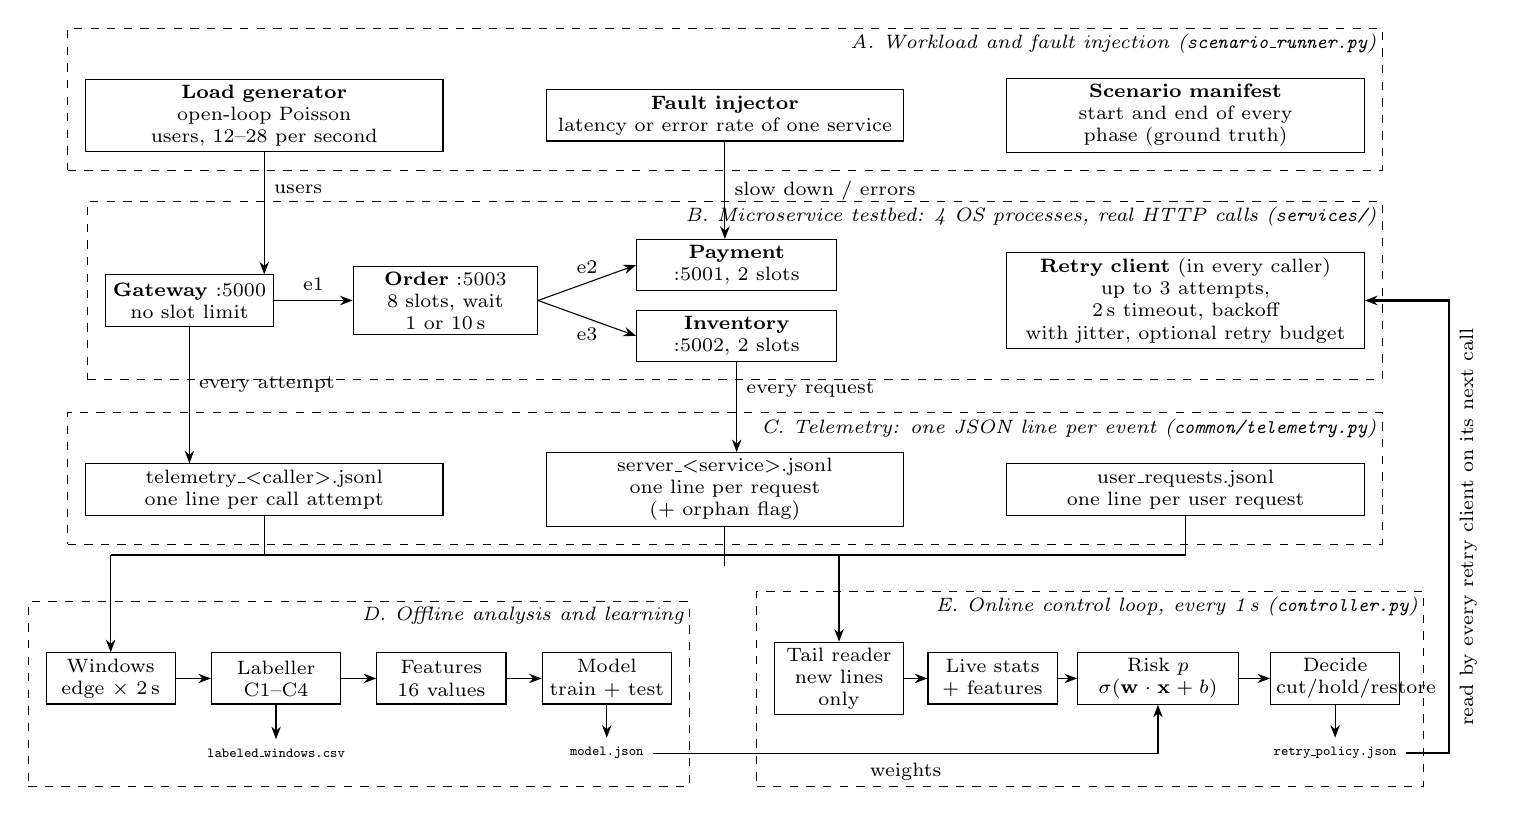
\begin{tikzpicture}[font=\scriptsize]
% ---- A: workload and fault injection
\node[blk, text width=44mm] (lg) at (2.9,0) {\textbf{Load generator}\\open-loop Poisson users, 12--28 per second};
\node[blk, text width=44mm] (fi) at (8.75,0) {\textbf{Fault injector}\\latency or error rate of one service};
\node[blk, text width=44mm] (mf) at (14.6,0) {\textbf{Scenario manifest}\\start and end of every phase (ground truth)};
% ---- B: testbed
\node[blk, text width=20mm] (gw) at (1.95,-2.35) {\textbf{Gateway} :5000\\no slot limit};
\node[blk, text width=22mm] (ord) at (5.2,-2.35) {\textbf{Order} :5003\\8 slots, wait 1 or 10\,s};
\node[blk, text width=24mm] (pay) at (8.9,-1.9) {\textbf{Payment} :5001, 2 slots};
\node[blk, text width=24mm] (inv) at (8.9,-2.8) {\textbf{Inventory} :5002, 2 slots};
\node[blk, text width=44mm] (rc) at (14.6,-2.35) {\textbf{Retry client} (in every caller)\\up to 3 attempts, 2\,s timeout, backoff\\with jitter, optional retry budget};
% ---- C: telemetry
\node[blk, text width=44mm] (t1) at (2.9,-4.75) {telemetry\_\textless caller\textgreater.jsonl\\one line per call attempt};
\node[blk, text width=44mm] (t2) at (8.75,-4.75) {server\_\textless service\textgreater.jsonl\\one line per request (+ orphan flag)};
\node[blk, text width=44mm] (t3) at (14.6,-4.75) {user\_requests.jsonl\\one line per user request};
% ---- D: offline
\node[blk, text width=15mm] (win) at (0.95,-7.15) {Windows\\edge $\times$ 2\,s};
\node[blk, text width=15mm] (lab) at (3.05,-7.15) {Labeller\\C1--C4};
\node[blk, text width=15mm] (fea) at (5.15,-7.15) {Features\\16 values};
\node[blk, text width=15mm] (mdl) at (7.25,-7.15) {Model\\train + test};
\node[font=\tiny\ttfamily] (lw) at (3.05,-8.1) {labeled\_windows.csv};
\node[font=\tiny\ttfamily] (mj) at (7.25,-8.1) {model.json};
% ---- E: online
\node[blk, text width=15mm] (tail) at (10.2,-7.15) {Tail reader\\new lines only};
\node[blk, text width=15mm] (live) at (12.15,-7.15) {Live stats\\+ features};
\node[blk, text width=19mm] (risk) at (14.25,-7.15) {Risk $p$\\$\sigma(\mathbf{w}\cdot\mathbf{x}+b)$};
\node[blk, text width=15mm] (dec) at (16.5,-7.15) {Decide\\cut/hold/restore};
\node[font=\tiny\ttfamily] (pol) at (16.5,-8.1) {retry\_policy.json};

% arrows
\draw[->] (lg.south) -- node[right, pos=0.3] {users} (lg.south |- gw.north);
\draw[->] (fi.south) -- node[right] {slow down / errors} (fi.south |- pay.north);
\draw[->] (gw) -- node[above] {e1} (ord);
\draw[->] (ord.east) -- node[above] {e2} (pay.west);
\draw[->] (ord.east) -- node[below] {e3} (inv.west);
\draw[->] (gw.south) -- node[right, pos=0.42] {every attempt} (gw.south |- t1.north);
\draw[->] (inv.south) -- node[right, pos=0.3] {every request} (inv.south |- t2.north);
% bus from telemetry to the two readers
\draw (t1.south) -- ++(0,-0.5) coordinate (b1);
\draw (t2.south) -- ++(0,-0.5);
\draw (t3.south) -- ++(0,-0.5) coordinate (b3);
\draw (b1 -| win.north) -- (b3);
\draw[->] (b1 -| win.north) -- (win.north);
\draw[->] (b1 -| tail.north) -- (tail.north);
% chains
\draw[->] (win) -- (lab);
\draw[->] (lab) -- (fea);
\draw[->] (fea) -- (mdl);
\draw[->] (lab) -- (lw);
\draw[->] (mdl) -- (mj);
\draw[->] (tail) -- (live);
\draw[->] (live) -- (risk);
\draw[->] (risk) -- (dec);
\draw[->] (dec) -- (pol);
\draw[->] (mj.east) -- node[below] {weights} (mj.east -| risk.south) -- (risk.south);
% feedback loop
\draw[->, thick] (pol.east) -- (17.95,-8.1) -- node[pos=0.5, sloped, below] {read by every retry client on its next call} (17.95,-2.35) -- (rc.east);

% layer boxes (a little headroom above each row for its label)
\path (lg.north) ++(0,0.42) coordinate (topA);
\path (rc.north) ++(0,0.42) coordinate (topB);
\path (t1.north) ++(0,0.42) coordinate (topC);
\path (win.north) ++(0,0.42) coordinate (topD);
\path (tail.north) ++(0,0.42) coordinate (topE);
\begin{scope}[on background layer]
\node[grp, fit=(lg)(fi)(mf)(topA)] (A) {};
\node[grp, fit=(gw)(ord)(pay)(inv)(rc)(topB)] (B) {};
\node[grp, fit=(t1)(t2)(t3)(topC)] (C) {};
\node[grp, fit=(win)(lab)(fea)(mdl)(lw)(mj)(topD)] (D) {};
\node[grp, fit=(tail)(live)(risk)(dec)(pol)(topE)] (E) {};
\end{scope}
\node[grplabel] at (A.north east) {A. Workload and fault injection (\texttt{scenario\_runner.py})};
\node[grplabel] at (B.north east) {B. Microservice testbed: 4 OS processes, real HTTP calls (\texttt{services/})};
\node[grplabel] at (C.north east) {C. Telemetry: one JSON line per event (\texttt{common/telemetry.py})};
\node[grplabel] at (D.north east) {D. Offline analysis and learning};
\node[grplabel] at (E.north east) {E. Online control loop, every 1\,s (\texttt{controller.py})};
\end{tikzpicture}
}
\caption{Overall architecture. (A) workload and fault injection, (B) the microservice testbed, (C) telemetry, (D) offline analysis and learning, (E) the online control loop. The thick arrow on the right closes the loop: every retry client reads the new \texttt{retry\_policy.json} on its next call.}
\label{fig:arch}
\end{figure*}

\subsection{Overview}
Fig.~\ref{fig:arch} shows the architecture in five layers. A load generator sends users to the gateway at a fixed Poisson rate (open loop: users keep arriving even when the system is slow). A fault injector changes only the faulty service's latency or error rate, and a manifest records the exact start and end of every phase, which serves as ground truth. Every call attempt and every received request is logged as one JSON line. Offline, the logs are cut into 2\,s windows per call edge, labelled with the four conditions, turned into 16 features, and used to train the model. Online, a controller reads the new log lines every second, computes the same features and the risk, and decides whether to cut, hold or restore the retry budget of each edge.

\subsection{Microservice Testbed}
The testbed (Fig.~\ref{fig:testbed}, Table~\ref{tab:params}) has four services, each a separate OS process running a Flask server that handles every request in its own thread. The gateway calls the order service, which calls the payment and inventory services. The three caller--callee links are the \emph{edges} e1--e3 that we monitor.

\begin{figure}[!t]
\centering
% testbed: four Flask processes, every arrow is an HTTP call with retries
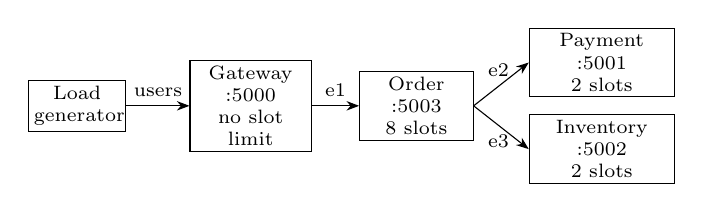
\begin{tikzpicture}[font=\scriptsize]
\node[blk, text width=11mm] (lg) {Load\\generator};
\node[blk, text width=14mm, right=8mm of lg] (gw) {Gateway\\:5000\\no slot limit};
\node[blk, text width=13mm, right=6mm of gw] (ord) {Order\\:5003\\8 slots};
\node[blk, text width=17mm, right=7mm of ord, yshift=5.5mm] (pay) {Payment :5001\\2 slots};
\node[blk, text width=17mm, right=7mm of ord, yshift=-5.5mm] (inv) {Inventory :5002\\2 slots};
\draw[->] (lg) -- node[above] {users} (gw);
\draw[->] (gw) -- node[above] {e1} (ord);
\draw[->] (ord.east) -- node[above, pos=0.45] {e2} (pay.west);
\draw[->] (ord.east) -- node[below, pos=0.45] {e3} (inv.west);
\end{tikzpicture}

\caption{Implemented testbed. Every arrow is an HTTP call with retries; e1--e3 are the monitored call edges.}
\label{fig:testbed}
\end{figure}

\begin{table}[!t]
\caption{Testbed Parameters}
\label{tab:params}
\centering
\small
\setlength{\tabcolsep}{4pt}
\begin{tabular}{|L{2.35cm}|L{1.15cm}|L{1.55cm}|L{1.65cm}|}
\hline
\textbf{Parameter} & \textbf{Gateway} & \textbf{Order} & \textbf{Payment / Inventory} \\ \hline
Worker slots $c$ & no limit & 8 & 2 \\ \hline
Own service time & -- & 10--40 ms & 30--90 ms \\ \hline
Built-in failure rate & -- & 2\% & 5\% \\ \hline
Longest wait for a slot & -- & 1 s or 10 s & 1 s \\ \hline
Retries on outgoing calls & 3 attempts & 3 attempts each & -- \\ \hline
\end{tabular}
\end{table}

Worker slots are modelled with a counting semaphore. A request must acquire a permit before doing its work and release it afterwards; if no permit becomes free within \texttt{queue\_wait\_sec} it is rejected with HTTP 503. Threads blocked in \texttt{acquire()} form the service's queue. The order service holds its slot while it calls payment and inventory, so a slow leaf also slows order. The wait limit of the order service is 1\,s by default and 10\,s in the ``long queue'' runs, which behave like a large thread-pool queue in a real server.

\subsection{Retry Client}
Every caller uses the same retry client. Up to three attempts are made with a 2\,s timeout each. Before attempt $k+1$ the client waits
\begin{equation}
d_k = h_k + \mathcal{U}(0,\, h_k), \qquad h_k = \frac{B\,2^{k-1}}{2}, \quad B = 100\text{ ms},
\label{eq:backoff}
\end{equation}
which is exponential backoff with equal jitter (50--100\,ms, then 100--200\,ms). A user gives up after 15\,s. For the retry-budget baseline the client keeps a token bucket per edge: each fresh call adds 0.1 token and each retry takes one, so retries cannot exceed about 10\% of fresh calls~\cite{brooker2019}. The retry policy of every edge is read from a small JSON file on every call, so a new policy takes effect immediately without restarting any service.

\subsection{Fault Injection}
Each service reads its configuration file (latency range, failure rate, slot wait) on every request. A scenario script changes only the faulty service's file. A gradual fault rises in steps: at severity $s \in [0,1]$ the latency range moves linearly from healthy (30--90\,ms) to the peak (for example 700--900\,ms). An error fault raises the failure rate instead. Services start from healthy settings, and a stopped run always removes its fault.

\subsection{Telemetry and Orphan Measurement}
Callers log one line per attempt (attempt number, response code with 0 for a timeout, latency, call id), services log one line per received request (arrival, slot time, status, deadline), and the load generator logs one line per user. Each attempt carries its deadline in an \texttt{X-Deadline} header. A service marks a request as orphaned when it finishes after that deadline. Fig.~\ref{fig:seq} shows how a retry creates orphaned work: attempt 1 waits in the order queue, the gateway gives up after 2\,s and sends attempt 2, and attempt 1 is later processed for nobody while holding a slot that a live request needed.

\begin{figure}[!t]
\centering
\resizebox{\columnwidth}{!}{% how a retry creates orphaned work (time goes down)
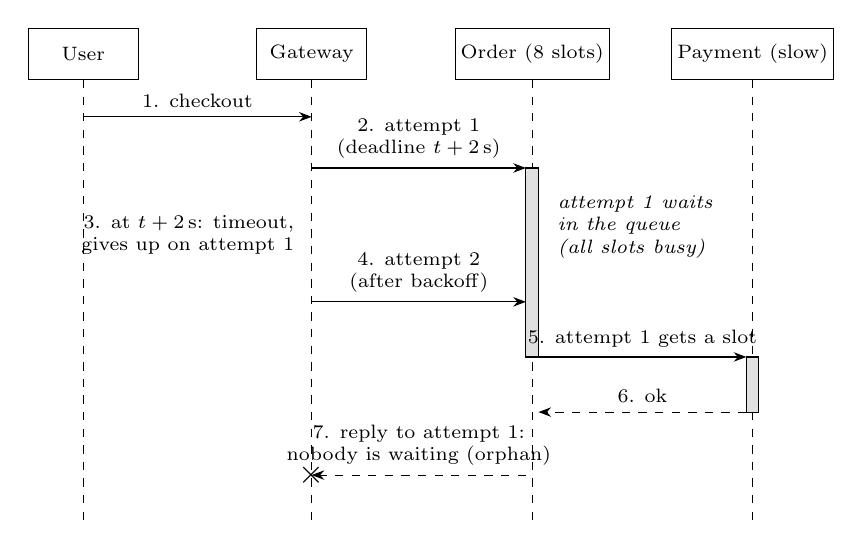
\begin{tikzpicture}[font=\scriptsize]
% lifelines
\foreach \x/\n/\t in {-0.3/u/User, 2.6/g/Gateway, 5.4/o/Order (8 slots), 8.2/p/Payment (slow)} {
  \node[blk, minimum width=14mm] (\n) at (\x,0) {\t};
  \draw[dashed, thin] (\n.south) -- (\x,-6.0);
}
% activation bars
\draw[fill=black!12] (5.32,-1.45) rectangle (5.48,-3.85);
\draw[fill=black!12] (8.12,-3.85) rectangle (8.28,-4.55);
% messages
\draw[->] (-0.3,-0.8) -- node[above] {1. checkout} (2.6,-0.8);
\draw[->] (2.6,-1.45) -- node[above, align=center] {2. attempt 1\\(deadline $t+2$\,s)} (5.32,-1.45);
\node[align=left, font=\scriptsize\itshape, anchor=west] at (5.6,-2.2) {attempt 1 waits\\in the queue\\(all slots busy)};
\node[align=right, anchor=east] at (2.5,-2.3) {3. at $t+2$\,s: timeout,\\gives up on attempt 1};
\draw[->] (2.6,-3.15) -- node[above, align=center] {4. attempt 2\\(after backoff)} (5.32,-3.15);
\draw[->] (5.48,-3.85) -- node[above] {5. attempt 1 gets a slot} (8.12,-3.85);
\draw[->, dashed] (8.12,-4.55) -- node[above] {6. ok} (5.48,-4.55);
\draw[->, dashed] (5.32,-5.35) -- node[above, align=center] {7. reply to attempt 1:\\nobody is waiting (orphan)} (2.6,-5.35);
\node at (2.6,-5.35) {\large$\times$};
\end{tikzpicture}
}
\caption{How a retry creates orphaned work during the fault (time goes down).}
\label{fig:seq}
\end{figure}

\subsection{Sharing Files Between Processes}
The controller writes the policy file while four services read it. To avoid partly written files, the writer writes a temporary file and replaces the real one with \texttt{os.replace}, which is atomic. On Windows the replace fails if another process has the file open, so it is retried up to 50 times. A reader that still fails keeps its last good policy.

\subsection{Offline Pipeline}
One command runs nine steps in order (Fig.~\ref{fig:pipe}): dataset generation, labelling, training with cross-validation, full evaluation, graph snapshots, experiments, labelling of the experiment runs, data validation and figures. Every number in this report comes from the files produced by these steps.

\begin{figure*}[!t]
\centering
% offline pipeline run by run_pipeline.py (9 steps, read in number order)
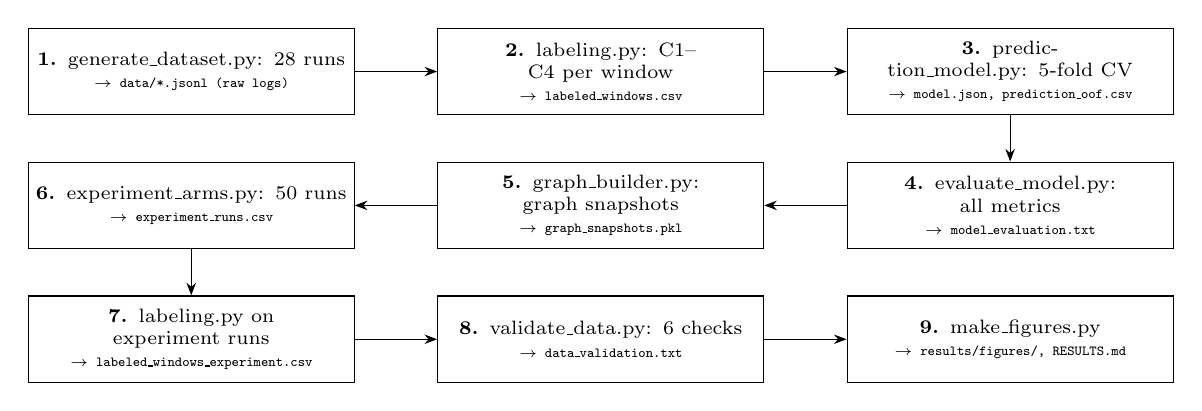
\begin{tikzpicture}[font=\scriptsize, stp/.style={blk, text width=40mm, minimum height=11mm}]
\node[stp] (s1) at (0,0)     {\textbf{1.} generate\_dataset.py: 28 runs\\\texttt{\tiny$\to$ data/*.jsonl (raw logs)}};
\node[stp] (s2) at (5.2,0)   {\textbf{2.} labeling.py: C1--C4 per window\\\texttt{\tiny$\to$ labeled\_windows.csv}};
\node[stp] (s3) at (10.4,0)  {\textbf{3.} prediction\_model.py: 5-fold CV\\\texttt{\tiny$\to$ model.json, prediction\_oof.csv}};
\node[stp] (s4) at (10.4,-1.7) {\textbf{4.} evaluate\_model.py: all metrics\\\texttt{\tiny$\to$ model\_evaluation.txt}};
\node[stp] (s5) at (5.2,-1.7)  {\textbf{5.} graph\_builder.py: graph snapshots\\\texttt{\tiny$\to$ graph\_snapshots.pkl}};
\node[stp] (s6) at (0,-1.7)    {\textbf{6.} experiment\_arms.py: 50 runs\\\texttt{\tiny$\to$ experiment\_runs.csv}};
\node[stp] (s7) at (0,-3.4)    {\textbf{7.} labeling.py on experiment runs\\\texttt{\tiny$\to$ labeled\_windows\_experiment.csv}};
\node[stp] (s8) at (5.2,-3.4)  {\textbf{8.} validate\_data.py: 6 checks\\\texttt{\tiny$\to$ data\_validation.txt}};
\node[stp] (s9) at (10.4,-3.4) {\textbf{9.} make\_figures.py\\\texttt{\tiny$\to$ results/figures/, RESULTS.md}};
\draw[->] (s1) -- (s2);
\draw[->] (s2) -- (s3);
\draw[->] (s3) -- (s4);
\draw[->] (s4) -- (s5);
\draw[->] (s5) -- (s6);
\draw[->] (s6) -- (s7);
\draw[->] (s7) -- (s8);
\draw[->] (s8) -- (s9);
\end{tikzpicture}

\caption{Offline pipeline run by \texttt{run\_pipeline.py}. Each step writes the files after the arrow; step 6 runs the controller with the model from step 3.}
\label{fig:pipe}
\end{figure*}

%====================================================================
\section{Why the Storm Sustains Itself}
\label{sec:mech}

During a payment slowdown to about 800\,ms, payment can finish at most $\mu = 2/0.8 = 2.5$ requests per second (Eq.~\ref{eq:queue}). Because order holds its slots while it waits for payment, order's throughput is capped at the same level. Users still arrive at 20 per second, order's queue fills, and requests that wait more than 2\,s are retried by the gateway. During the fault every strategy in our experiments served only 5--6\% of users; no retry policy can create capacity.

The difference appears after the fault. Just after recovery, order can finish about $\mu \approx 8/0.25 \approx 32$ requests per second (0.25\,s instead of the healthy 0.2\,s because the leaves are still busy with queued work). With a backlog of about 200 requests, the queue wait is about 6\,s, longer than the 2\,s timeout, so almost every request that gets a slot has already been abandoned. Its user fails and the gateway retries, so with three attempts up to $3 \times 20 = 60$ requests per second arrive. The backlog can only drain if
\begin{equation}
\lambda \cdot a < \mu
\label{eq:exit}
\end{equation}
where $a$ is the number of attempts each user causes. Here $20 \times 3 = 60 > 32$, while $20 \times 1 = 20 < 32$.
So with three attempts the backlog never drains and the stuck state sustains itself. With one attempt it drains at $32-20=12$ requests per second, about 16\,s for 200 requests; we measured 11.4\,s for the no-retry strategy.

The slot wait decides whether this can happen. With a 1\,s wait, a request that cannot get a slot is rejected with 503 \emph{before} the gateway's 2\,s timeout, nothing stale stays in the queue, and the storm ends with the fault (\emph{fault-coupled} livelock). With a 10\,s wait, abandoned requests stay queued and are processed later for nobody, which makes the storm \emph{self-sustaining}.

%====================================================================
\section{Dataset}
\label{sec:data}

\subsection{Why a Public Dataset Could Not Be Used}
Labelling retry livelock needs three things for every call: which attempt it was, its outcome, and when the fault started and ended. Table~\ref{tab:datasets} shows that no public dataset has all three. The closest source, the OSDI 2022 metastability work~\cite{huang2022}, is a method rather than a dataset: it runs a real system and injects a trigger, which is what we do.

\begin{table}[!t]
\caption{Public Datasets Examined}
\label{tab:datasets}
\centering
\small
\begin{tabular}{|L{2.6cm}|L{1.15cm}|L{1.3cm}|L{1.3cm}|}
\hline
\textbf{Dataset} & \textbf{Attempt no.} & \textbf{Outcome} & \textbf{Fault timing} \\ \hline
Alibaba traces 2021~\cite{alibaba2021} & No & No (RT only) & No \\ \hline
Alibaba traces 2022 & No & No & No \\ \hline
Meta traces~\cite{meta2023} & No & No & No \\ \hline
Uber error data~\cite{lee2024} & No & Partly & No \\ \hline
RCAEval~\cite{rcaeval2024} & No & Partly & Yes \\ \hline
OSDI 2022 method~\cite{huang2022} & Yes & Yes & Yes (method) \\ \hline
\end{tabular}
\end{table}

\subsection{Generation}
The generator draws 24 scenarios from a seeded random generator (seed 7) over six factors: fault kind (latency 60\%, error 40\%), target (payment 60\%, inventory 40\%), order slot wait (1\,s, or 4, 6, 8 or 10\,s), load (12--22 users/s), fault shape (gradual ramp of 3--6 steps over 6--14\,s, or a sudden spike) and severity (peak latency 500--900\,ms or peak error rate 60--90\%). Four control runs have no fault at all, two of them at high load (26 and 28 users/s), to test that the detector does not fire on a merely busy system. All dataset runs use the static three-attempt policy so that the model sees storms that nothing stops. Each run has a healthy phase of 10--12\,s, a ramp or spike, a held fault of 6--12\,s and a recovery phase of 15--20\,s. The 28 runs took 22.9 minutes. With the 50 experiment runs the data holds 78 runs, 263,864 call attempts, 71,621 user requests and 335,485 server records.

Only the fault is injected. Retries, queue build-up, amplification and collapse are never scripted; they come from the running system.

\subsection{Validation}
A validation script checks six properties that must hold if the testbed behaves like a real system, and all six pass:
\begin{enumerate}
\item \emph{Bookkeeping}: every user request sent is logged, and every request a service received equals a first attempt its caller logged (largest gap 0).
\item \emph{Retry rules}: over 218,897 logical calls, attempts are numbered $1..k$ in order, never exceed the policy limit, and a call is never retried after success.
\item \emph{Queueing theory}: no service is ever more than 100\% busy in any 2\,s window ($U \le 1$), and under a held latency fault the measured throughput is 91\% of $c/S$ on average, so the service is saturated.
\item \emph{Fault injection}: measured service times and failure fractions match the configured values (bias +0.4\%); healthy leaves fail 5.0\% of requests.
\item \emph{Load generator}: the arrival rate is within 2.5\% of the target on average.
\item \emph{Timestamps}: none of 670,970 records ends before it starts.
\end{enumerate}
Regenerating the whole dataset three times gave 132, 135 and 131 livelock windows.

%====================================================================
\section{Livelock Detection}
\label{sec:detect}

\subsection{Window Statistics}
For each edge $e$ and 2\,s window $w$ (length $\Delta$) we count, over the attempts that \emph{ended} in the window, the fresh calls $n_f$ (attempt 1), the retries $n_r$, the successes $n_s$, and the 503 and timeout replies. From these:
\begin{gather}
\lambda_{\text{base}} = \frac{n_f}{\Delta}, \quad \lambda_{\text{retry}} = \frac{n_r}{\Delta}, \quad \rho = \frac{n_r}{n_f}, \\
S = \frac{n_s}{\Delta}, \quad P = \frac{n_s}{n_f+n_r},
\end{gather}
with $\rho$ capped at 10. The number of calls in flight $N$ is a time average computed from exact start and end times:
\begin{equation}
N(w) = \frac{1}{\Delta} \sum_i \bigl|\,[t^{\text{start}}_i, t^{\text{end}}_i] \cap w\,\bigr| .
\end{equation}
The healthy levels $S^\ast$ and $N^\ast$ of each edge are the medians over the first 8\,s of the same run, so every edge is compared with itself.

\subsection{The Four Conditions}
A window satisfies:
\begin{align}
\text{C1:}\;& \rho > 1 \label{eq:c1}\\
\text{C2:}\;& S < 0.5\, S^\ast \\
\text{C3:}\;& N > \max(2N^\ast, 1) \;\wedge\; N(w) \ge 0.8\, N(w-2) \\
\text{C4:}\;& \lambda_{\text{retry}}(w) \ge 0.8\,\lambda_{\text{retry}}(w-2) \;\wedge\; P(w) \le P(w-2) + 0.05 \label{eq:c4}
\end{align}
An edge is in livelock in window $w$ when all four hold for two windows in a row and the window has at least four calls. C1 (more retries than fresh calls) and C4 (the retry loop is not dying out) separate livelock from overload; an overloaded system without retries fails C1. C2 and C3 express that there is no progress and that work is stuck inside the system. The 20\% tolerance in C3 and C4 prevents random up-and-down movement in a steady storm from switching the conditions off.

\subsection{Detection Results}
Table~\ref{tab:detect} shows the result on the 28 dataset runs: 131 livelock windows out of 1,878, almost all on gateway$\to$order, during the fault and the recovery, and 0 false alarms in 636 healthy windows, including the high-load controls. The label matches what users experienced: users who arrived in a flagged window succeeded 9.0\% of the time, against 68.1\% in other fault and recovery windows. Fig.~\ref{fig:ds06} shows one run in detail. The storm appears on gateway$\to$order rather than on the faulty leaf because order's eight slots cap how many retries can pile up towards the leaf, while the gateway has no limit; per-edge analysis points at where the storm is, not where the fault is.

\begin{table}[!t]
\caption{Livelock Windows by Edge and Phase (28 Dataset Runs)}
\label{tab:detect}
\centering
\small
\begin{tabular}{|l|c|c|c|c|}
\hline
\textbf{Edge} & \textbf{Normal} & \textbf{Ramp} & \textbf{Fault} & \textbf{Recovery} \\ \hline
gateway$\to$order & 0/212 & 8/93 & 46/104 & 63/209 \\ \hline
order$\to$payment & 0/212 & 0/93 & 1/104 & 0/209 \\ \hline
order$\to$inventory & 0/212 & 1/93 & 9/104 & 0/209 \\ \hline
\end{tabular}
\end{table}

\begin{figure}[!t]
\centering
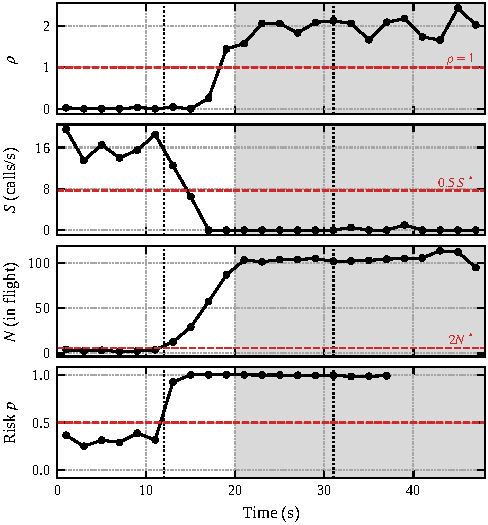
\includegraphics[width=\columnwidth]{plot_detection.pdf}
\caption{Run ds\_06, edge gateway$\to$order, one point per 2\,s window. $\rho$ rises above 1 and stays near 2, useful throughput $S$ falls to 0, and calls in flight $N$ exceed 100. Grey bands are livelock windows; they continue after the fault is removed (second dotted line). Dashed lines are the thresholds of C1--C3 and the risk threshold 0.5; the risk crossed 0.5 about 8\,s before the first livelock window.}
\label{fig:ds06}
\end{figure}

\subsection{Threshold Sensitivity}
Because the labels come from our own definition, we moved each threshold up and down and relabelled everything (Table~\ref{tab:sens}). False alarms stayed at 0 for every setting and the counts change smoothly. The trend tolerance matters most: with no tolerance (our earlier version) only 45 of the 128 storm windows are found.

\begin{table}[!t]
\caption{Sensitivity of the Labels (Windows in Ramp, Fault and Recovery)}
\label{tab:sens}
\centering
\small
\begin{tabular}{|L{1.6cm}|L{0.7cm}|L{1.9cm}|L{1.75cm}|}
\hline
\textbf{Parameter} & \textbf{Used} & \textbf{Values tried} & \textbf{Livelock windows} \\ \hline
$\rho$ limit (C1) & 1.0 & 0.5, 0.75, 1, 1.25, 1.5 & 156, 139, 128, 119, 97 \\ \hline
$\beta$ (C2) & 0.5 & 0.3, 0.4, 0.5, 0.6, 0.7 & 123, 124, 128, 132, 139 \\ \hline
C factor (C3) & 2.0 & 1.5, 2, 3, 4 & 128, 128, 128, 118 \\ \hline
Trend tolerance & 0.2 & 0, 0.1, 0.2, 0.3 & 45, 94, 128, 153 \\ \hline
Windows in a row & 2 & 1, 2, 3, 4 & 183, 128, 93, 66 \\ \hline
\multicolumn{4}{|l|}{False alarms: 0 of 636 healthy windows at every value.} \\ \hline
\end{tabular}
\end{table}

%====================================================================
\section{Livelock Prediction}
\label{sec:predict}

\subsection{Task}
Every 2\,s, for every edge, the model answers: will this edge be in livelock in any of the next five windows, that is 2--12\,s after the current window starts? The current window is not part of the label, so the task is prediction rather than detection. The dataset gives 1,458 examples from 28 runs, of which 216 (14.8\%) are positive.

\subsection{Features}
Table~\ref{tab:feat} lists the 16 features. The graph features are one round of message passing over the service graph: each edge receives the worst overload, latency ratio and failure ratio among the edges directly below it, and the $\rho$ and overload of the edge directly above it. A slowdown begins at a leaf, but the storm forms at the top, so these features carry the early sign upwards. The same code computes the features offline, in training and in the live controller.

\begin{table}[!t]
\caption{The 16 Features}
\label{tab:feat}
\centering
\small
\begin{tabular}{|L{1.35cm}|L{6.2cm}|}
\hline
\textbf{Group} & \textbf{Features} \\ \hline
Own edge (5) & $\rho$; fresh-call failure ratio; overload ratio (503 + timeouts); latency and calls in flight relative to the edge's healthy level \\ \hline
Temporal (3) & change of $\rho$, failure ratio and latency ratio since the previous window \\ \hline
Graph (5) & worst overload, latency ratio and failure ratio among the edges below; $\rho$ and overload of the edge above \\ \hline
Edge id (3) & one-hot: gateway$\to$order, order$\to$payment, order$\to$inventory \\ \hline
\end{tabular}
\end{table}

\subsection{Model}
We use logistic regression. Features are standardised with the training mean $m_j$ and standard deviation $s_j$, and the risk is
\begin{equation}
p = \sigma\!\Bigl(b + \sum_{j=1}^{16} w_j \frac{x_j - m_j}{s_j}\Bigr), \qquad \sigma(z) = \frac{1}{1+e^{-z}} .
\label{eq:lr}
\end{equation}
The weights minimise the class-weighted log loss with an L2 penalty ($C=1$):
\begin{equation}
L = -\sum_i \omega_{y_i}\bigl[y_i \ln p_i + (1-y_i)\ln(1-p_i)\bigr] + \frac{1}{2C}\lVert \mathbf{w} \rVert^2,
\end{equation}
with $\omega_1 = n/(2n_+) \approx 3.4$ and $\omega_0 = n/(2n_-) \approx 0.59$, so the rare positive class counts as much as the negative class. We chose logistic regression on purpose. The trained model is 49 numbers (16 means, 16 standard deviations, 16 weights and the bias) stored in a 2.2\,KB file, and the controller computes Eq.~\ref{eq:lr} with its own code every second. On all 1,458 examples the hand-computed risk equals the library's to within $3.3\times10^{-16}$. The decision threshold is 0.5, fixed before evaluation. The largest weights are the fresh-call failure ratio ($+1.89$), the overload ratio ($-1.65$), the calls-in-flight ratio ($+1.53$) and the worst latency ratio below ($+1.52$). Because the features are correlated, single weights are not read on their own; feature groups are judged by ablation.

\subsection{Evaluation Protocol}
Neighbouring windows of one run are nearly copies of each other, so a random split would leak the answer. We use 5-fold cross-validation \emph{grouped by run}: all windows of a run are in the same fold, and every window receives an out-of-fold risk from a model that never saw its run. The standardiser is fitted on the training folds only. We compare against a reactive rule ($\rho > 1$ and overload $> 20\%$ now), a persistence rule (livelock soon if livelock now), ablations without graph or temporal features, a random forest (200 trees, depth 6), and a control trained on shuffled labels. We also score the \emph{before-onset} subset (the edge is not in livelock now or in the previous window; 1,341 examples, 123 positive), which is the case pre-emption needs, and we measure the lead time before each of the 30 livelock episodes.

\subsection{Results}
Table~\ref{tab:cm} gives the confusion matrix of our model and Table~\ref{tab:metrics} every metric computed from it. The Matthews correlation coefficient uses all four cells,
\begin{equation}
\text{MCC} = \frac{TP\cdot TN - FP\cdot FN}{\sqrt{(TP+FP)(TP+FN)(TN+FP)(TN+FN)}},
\label{eq:mcc}
\end{equation}
and is 0 for guessing and 1 for a perfect model. All metrics are computed by our own code from the four cells and cross-checked against scikit-learn. The model reaches 91.8\% accuracy, 88.9\% balanced accuracy and MCC 0.71. Accuracy alone is not enough here: 85.2\% of windows are negative, so always answering ``no'' is already 85.2\% accurate but has balanced accuracy 50\% and MCC 0. Precision (68.0\%) is lower than recall (84.7\%) by design: a missed storm can leave the system stuck, while an unneeded alarm costs at most one early cut that the controller later restores.

\begin{table}[!t]
\caption{Confusion Matrix of Our Model (1,458 Out-of-Fold Windows, Threshold 0.5)}
\label{tab:cm}
\centering
\small
\begin{tabular}{|l|c|c|}
\hline
 & \textbf{Predicted: no} & \textbf{Predicted: yes} \\ \hline
\textbf{Actual: no} (1,242) & TN = 1,156 & FP = 86 \\ \hline
\textbf{Actual: yes} (216) & FN = 33 & TP = 183 \\ \hline
\end{tabular}
\end{table}

\begin{table}[!t]
\caption{Metrics Computed From the Confusion Matrix}
\label{tab:metrics}
\centering
\small
\setlength{\tabcolsep}{4pt}
\begin{tabular}{|L{1.75cm}|L{3.95cm}|L{1.45cm}|}
\hline
\textbf{Metric} & \textbf{Formula and numbers} & \textbf{Value} \\ \hline
Accuracy & $(TP+TN)/n$ = 1339/1458 & 91.8\% \\ \hline
Precision & $TP/(TP+FP)$ = 183/269 & 68.0\% \\ \hline
Recall & $TP/(TP+FN)$ = 183/216 & 84.7\% \\ \hline
Specificity & $TN/(TN+FP)$ = 1156/1242 & 93.1\% \\ \hline
Balanced acc. & $(\text{Rec.}+\text{Spec.})/2$ & 88.9\% \\ \hline
F1 / F2 & $2PR/(P+R)$; $5PR/(4P+R)$ & 75.5\% / 80.8\% \\ \hline
MCC & Eq.~(\ref{eq:mcc}), uses all four cells & 0.71 \\ \hline
Cohen's $\kappa$ & agreement beyond chance & 0.71 \\ \hline
ROC-AUC & P(positive ranked above negative) & 0.95 \\ \hline
PR-AUC & area under precision--recall (chance 0.15) & 0.84 \\ \hline
Brier / ECE & mean $(p-y)^2$; calibration gap & 0.072 / 0.10 \\ \hline
\end{tabular}
\end{table}

Table~\ref{tab:pred} compares the methods. On all windows our model reaches F1 0.75 and PR-AUC 0.84. Before onset the persistence rule scores 0 and the reactive rule 0.32, while our model scores 0.66. The graph features matter most there (PR-AUC 0.74 with them, 0.63 without); the temporal features add nothing measurable. The random forest is a little better (F1 0.80) but, as shown below, far more expensive. The shuffled-label control is at chance, so the setup does not leak the answer.

\begin{table*}[!t]
\caption{Prediction Results, 5-Fold Cross-Validation Grouped by Run (Last Three Columns: Before Onset Only)}
\label{tab:pred}
\centering
\small
\setlength{\tabcolsep}{4pt}
\begin{tabular}{|l|c|c|c|c|c|c||c|c|c|}
\hline
\textbf{Method} & \textbf{Acc.} & \textbf{Bal. acc.} & \textbf{Prec.} & \textbf{Recall} & \textbf{F1} & \textbf{MCC} & \textbf{F1 (onset)} & \textbf{MCC (onset)} & \textbf{PR-AUC (onset)} \\ \hline
Logistic regression (ours) & 0.92 & 0.89 & 0.68 & 0.85 & 0.75 & 0.71 & 0.66 & 0.63 & 0.74 \\ \hline
\quad without graph features & 0.91 & 0.88 & 0.66 & 0.84 & 0.74 & 0.70 & 0.63 & 0.59 & 0.63 \\ \hline
\quad without temporal features & 0.91 & 0.89 & 0.66 & 0.85 & 0.75 & 0.70 & 0.64 & 0.61 & 0.73 \\ \hline
Random forest (comparison) & 0.94 & 0.90 & 0.76 & 0.84 & 0.80 & 0.76 & 0.70 & 0.67 & 0.79 \\ \hline
Rule: storm now (reactive) & 0.90 & 0.74 & 0.72 & 0.52 & 0.60 & 0.56 & 0.32 & 0.30 & -- \\ \hline
Rule: livelock now (persistence) & 0.90 & 0.69 & 0.87 & 0.38 & 0.53 & 0.54 & 0.00 & 0.00 & -- \\ \hline
Shuffled-label control & 0.47 & 0.40 & 0.09 & 0.29 & 0.14 & $-$0.15 & 0.11 & $-$0.09 & 0.09 \\ \hline
\end{tabular}
\end{table*}

\textbf{Early warning.} The model warned before all 30 livelock episodes with a median lead of 8\,s (range 2--10\,s); the reactive rule warned before 24 with a median of 2\,s (Fig.~\ref{fig:lead}). The cost is alarms in 8 of 576 healthy windows (1.4\%). Fig.~\ref{fig:graph} shows why the graph features help: at 12\,s the gateway$\to$order edge already has risk 0.92 while its own $\rho$ is only 0.04, because the slowdown is visible first on the edges below it.

\begin{figure}[!t]
\centering
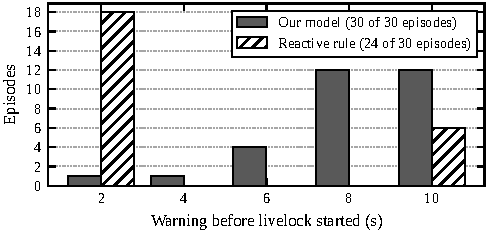
\includegraphics[width=\columnwidth]{plot_lead_time.pdf}
\caption{Seconds of warning before each of the 30 livelock episodes.}
\label{fig:lead}
\end{figure}

\begin{figure*}[!t]
\centering
\resizebox{\textwidth}{!}{% three snapshots of the service graph, run ds_06 (values from graph_builder.py)
% thin = normal, dashed = predicted risk >= 0.5, very thick = livelock (C1-C4 hold)
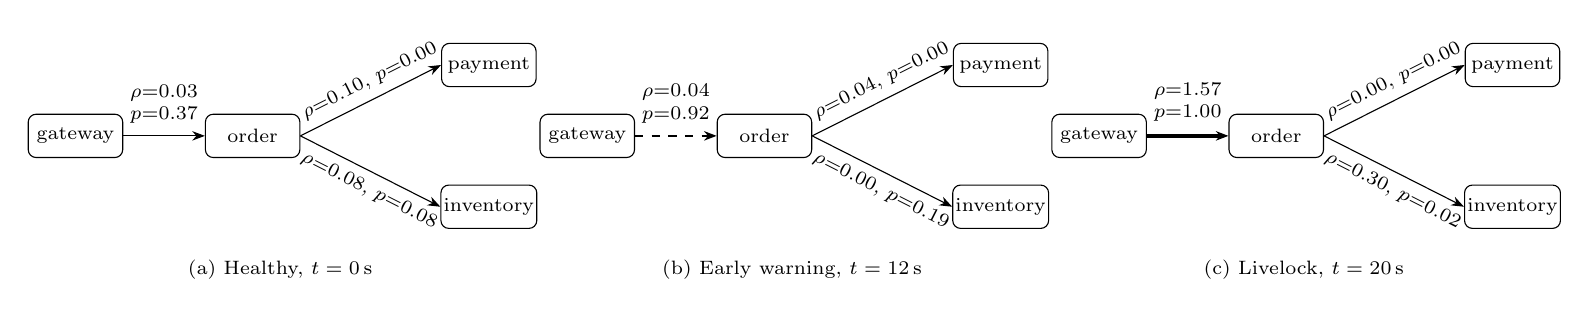
\begin{tikzpicture}[font=\scriptsize,
  svc/.style={draw, rounded corners=1mm, minimum width=12mm, minimum height=5.5mm, inner sep=1pt, font=\scriptsize},
  normal/.style={->, thin},
  warn/.style={->, thick, dashed},
  lock/.style={->, line width=1.6pt}]
\foreach \dx/\cap/\sa/\sb/\sc/\la/\lb/\lc in {
  0/{(a) Healthy, $t=0$\,s}/normal/normal/normal/{$\rho$=0.03\\$p$=0.37}/{$\rho$=0.10, $p$=0.00}/{$\rho$=0.08, $p$=0.08},
  6.5/{(b) Early warning, $t=12$\,s}/warn/normal/normal/{$\rho$=0.04\\$p$=0.92}/{$\rho$=0.04, $p$=0.00}/{$\rho$=0.00, $p$=0.19},
  13.0/{(c) Livelock, $t=20$\,s}/lock/normal/normal/{$\rho$=1.57\\$p$=1.00}/{$\rho$=0.00, $p$=0.00}/{$\rho$=0.30, $p$=0.02}} {
  \begin{scope}[xshift=\dx cm]
    \node[svc] (g) at (0,0) {gateway};
    \node[svc] (o) at (2.25,0) {order};
    \node[svc] (p) at (5.25,0.9) {payment};
    \node[svc] (i) at (5.25,-0.9) {inventory};
    \draw[\sa] (g) -- node[above=1pt, font=\scriptsize, align=center] {\la} (o);
    \draw[\sb] (o.east) -- node[above, pos=0.55, font=\scriptsize, sloped] {\lb} (p.west);
    \draw[\sc] (o.east) -- node[below, pos=0.55, font=\scriptsize, sloped] {\lc} (i.west);
    \node at (2.6,-1.7) {\cap};
  \end{scope}
}
\end{tikzpicture}
}
\caption{Three snapshots of the service graph for run ds\_06, with $\rho$ and the predicted risk $p$ on every edge (values from \texttt{graph\_builder.py}). Thin arrow: normal; dashed: $p \ge 0.5$; thick: livelock (C1--C4 hold). At 12\,s gateway$\to$order already has risk 0.92 while its own $\rho$ is only 0.04.}
\label{fig:graph}
\end{figure*}

\textbf{Curves and calibration.} Fig.~\ref{fig:eval} shows the ROC and precision--recall curves, the calibration curve and the effect of the threshold. Class weighting pushes the risk values above the true frequencies (risks of 0.5--0.9 were followed by livelock 35--53\% of the time, ECE 0.10). This does not change the ranking (ROC-AUC 0.95), and the threshold was fixed for this model. Moving the threshold to 0.6 would give F1 0.76, but choosing a threshold on the data we report on would inflate the result, so we keep 0.5.

\begin{figure}[!t]
\centering
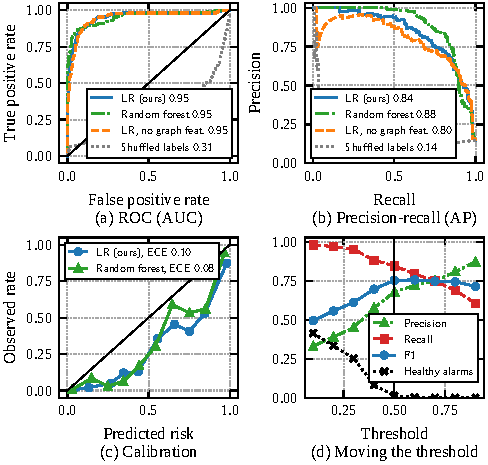
\includegraphics[width=\columnwidth]{plot_model_eval.pdf}
\caption{Out-of-fold evaluation on 1,458 windows: (a) ROC, (b) precision--recall, (c) calibration, (d) effect of the threshold (vertical line: 0.5, the threshold used). LR: logistic regression.}
\label{fig:eval}
\end{figure}

\textbf{Confidence intervals.} We resampled the 28 runs with replacement 1,000 times and recomputed each metric (Table~\ref{tab:boot}). Whole runs are resampled because windows of one run are not independent. The gains over the reactive rule and from the graph features stay above zero, so they are not due to chance.

\begin{table}[!t]
\caption{95\% Bootstrap Intervals (1,000 Resamples of Whole Runs)}
\label{tab:boot}
\centering
\small
\begin{tabular}{|L{4.1cm}|c|c|}
\hline
\textbf{Quantity} & \textbf{Value} & \textbf{95\% interval} \\ \hline
F1, all windows & 0.75 & 0.64 to 0.83 \\ \hline
MCC, all windows & 0.71 & 0.61 to 0.79 \\ \hline
ROC-AUC, all windows & 0.95 & 0.90 to 0.98 \\ \hline
PR-AUC, all windows & 0.84 & 0.75 to 0.91 \\ \hline
F1 gain over reactive rule, before onset & +0.34 & +0.23 to +0.42 \\ \hline
PR-AUC gain from graph features, before onset & +0.10 & +0.02 to +0.19 \\ \hline
PR-AUC gap to the random forest & $-$0.04 & $-$0.07 to $-$0.02 \\ \hline
\end{tabular}
\end{table}

\textbf{Where it works.} The model is best on the case it was built for: latency faults (F1 0.87, MCC 0.84) and long slot waits (F1 0.85, MCC 0.82). It is weaker on error faults (F1 0.59), where storms are short. The order$\to$payment edge has only 5 positive windows in the whole dataset, too few to learn or judge. On the no-fault control runs it raised 6 false alarms in 180 windows.

\textbf{Run-time cost.} Table~\ref{tab:cost} shows why we kept logistic regression. One prediction takes 5.2\,$\mu$s with our own code and a whole controller round 30.3\,$\mu$s, which is 0.003\% of its 1\,s interval. The random forest needs 12,837\,$\mu$s per prediction, about 2,500 times more, and is over 400 times larger, for a PR-AUC gain of 0.04.

\begin{table}[!t]
\caption{Run-Time Cost (Measured on the Pipeline Machine)}
\label{tab:cost}
\centering
\small
\setlength{\tabcolsep}{4pt}
\begin{tabular}{|L{2.45cm}|L{2.55cm}|L{2.0cm}|}
\hline
\textbf{Item} & \textbf{Logistic regression} & \textbf{Random forest} \\ \hline
One prediction & 5.2 $\mu$s (own code) & 12,837 $\mu$s \\ \hline
Controller round (3 edges) & 30.3 $\mu$s & -- \\ \hline
Training (1,458 windows) & 15 ms & 449 ms \\ \hline
Model size & 49 numbers, 2.2 KB & 200 trees, about 1 MB \\ \hline
\end{tabular}
\end{table}

%====================================================================
\section{Retry-Budget Controller}
\label{sec:control}

\subsection{Control Loop}
The controller runs every second (Fig.~\ref{fig:flow}). It reads only the lines appended to the call logs since its last check, using remembered byte offsets, keeps the last 4\,s of attempts, and computes the statistics of the last 2\,s and of the 2\,s before that for every edge. In predictive mode it builds the 16 features with the same code as training and computes the risk with Eq.~\ref{eq:lr}.

\begin{figure}[!t]
\centering
% one control step, done for every edge every second (controller.py)
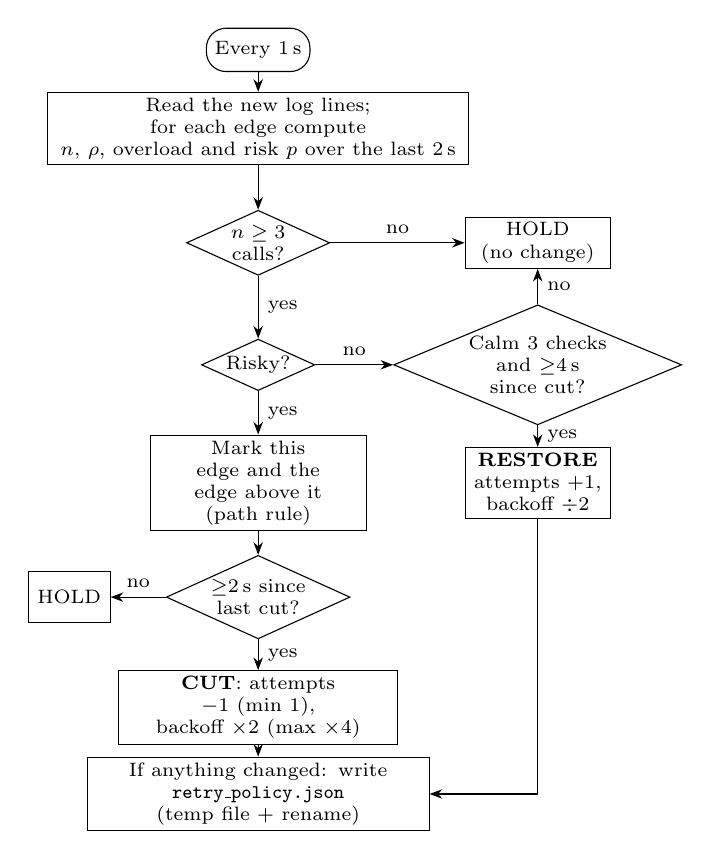
\begin{tikzpicture}[font=\scriptsize]
\node[term] (st) at (0,0) {Every 1\,s};
\node[blk, text width=52mm] (rd) at (0,-1.0) {Read the new log lines; for each edge compute\\$n$, $\rho$, overload and risk $p$ over the last 2\,s};
\node[dec] (d1) at (0,-2.45) {$n \ge 3$\\calls?};
\node[blk, text width=17mm] (h1) at (3.55,-2.45) {HOLD\\(no change)};
\node[dec] (d2) at (0,-4.0) {Risky?};
\node[dec, aspect=2.4] (d3) at (3.55,-4.0) {Calm 3 checks\\and $\ge$4\,s\\since cut?};
\node[blk, text width=26mm] (mk) at (0,-5.5) {Mark this edge and the\\edge above it (path rule)};
\node[blk, text width=17mm] (rs) at (3.55,-5.5) {\textbf{RESTORE}\\attempts $+1$,\\backoff $\div 2$};
\node[dec] (d4) at (0,-6.95) {$\ge$2\,s since\\last cut?};
\node[blk, text width=9mm] (h2) at (-2.4,-6.95) {HOLD};
\node[blk, text width=34mm] (ct) at (0,-8.35) {\textbf{CUT}: attempts $-1$ (min 1),\\backoff $\times 2$ (max $\times 4$)};
\node[blk, text width=42mm] (wr) at (0,-9.45) {If anything changed: write\\\texttt{retry\_policy.json} (temp file + rename)};

\draw[->] (st) -- (rd);
\draw[->] (rd) -- (d1);
\draw[->] (d1) -- node[above] {no} (h1);
\draw[->] (d1) -- node[right] {yes} (d2);
\draw[->] (d2) -- node[above] {no} (d3);
\draw[->] (d3) -- node[right] {no} (h1);
\draw[->] (d3) -- node[right] {yes} (rs);
\draw[->] (d2) -- node[right] {yes} (mk);
\draw[->] (mk) -- (d4);
\draw[->] (d4) -- node[above] {no} (h2);
\draw[->] (d4) -- node[right] {yes} (ct);
\draw[->] (ct) -- (wr);
\draw[->] (rs.south) -- (rs.south |- wr.east) -- (wr.east);
\end{tikzpicture}

\caption{One control step, done for every edge every second. Risky: ($p \ge 0.5$ and congestion starting on or below the edge) or ($\rho > 1$ and overload $> 0.2$), Eq.~\ref{eq:risky}.}
\label{fig:flow}
\end{figure}

\subsection{Decision Rule}
An edge with at least three calls in the window is \emph{risky} when
\begin{equation}
\underbrace{(p_e \ge 0.5 \;\wedge\; G_e)}_{\text{predicted}} \;\vee\; \underbrace{(\rho_e > 1 \;\wedge\; o_e > 0.2)}_{\text{reactive safety net}},
\label{eq:risky}
\end{equation}
where $o_e$ is the overload ratio and $G_e$ (the \emph{congestion gate}) is true when overload is at least 10\% on the edge or an edge below it, or the callee's response time is at least twice its healthy level. For gateway$\to$order the gate looks at the latency of the edges below, because order's own response time includes its retry backoff, which is not congestion. Reactive mode uses only the second term.

\subsection{Cut, Restore and the Path Rule}
A risky edge is cut: the number of attempts drops by one (minimum 1) and the backoff base doubles (maximum four times the original), at most once every 2\,s. Because retries multiply down a chain, the edge \emph{above} a risky edge is cut as well (the path rule). An edge that is not risky gives back one step (one attempt, backoff halved) only after it has been free of overload ($o_e < 0.1$) for three checks in a row and at least 4\,s have passed since its last cut. This is additive-increase/multiplicative-decrease (AIMD) in spirit, as in TCP congestion control: react quickly to congestion, give back slowly.

The restore condition uses overload, not $\rho$. When attempts are cut to one, $\rho$ is zero by definition, so a rule that restores on low $\rho$ gives retries back while the callee is still overloaded, and the controller oscillates. Our earlier version had exactly this problem. Overload is measured on fresh calls as well, so it remains meaningful with retries off.

When the controller stops, it writes the original policy back so that the services are never left with retries switched off. Algorithm~\ref{alg:ctrl} summarises one step.

\begin{algorithm}[!t]
\caption{One Control Step (Every 1 s)}
\label{alg:ctrl}
\begin{algorithmic}[1]
\State $R \gets$ new call records since the last step (tail read)
\For{each edge $e$}
  \State compute stats of the last 2\,s and the previous 2\,s
  \State $p_e \gets$ risk from Eq.~(\ref{eq:lr}) \Comment{predictive mode}
  \State $\textit{risky}_e \gets n_e \ge 3 \wedge$ Eq.~(\ref{eq:risky})
\EndFor
\State $\textit{Cut} \gets \{e : \textit{risky}_e\} \cup \{\text{parent}(e) : \textit{risky}_e\}$
\For{each edge $e$}
  \If{$e \in \textit{Cut}$ and $t - t^{\text{cut}}_e \ge 2$\,s}
    \State $a_e \gets \max(1, a_e - 1)$;\; $\beta_e \gets \min(4, 2\beta_e)$;\; $t^{\text{cut}}_e \gets t$
  \ElsIf{$e \notin \textit{Cut}$}
    \State update calm counter $h_e$ (calm: $n_e \ge 3$ and $o_e < 0.1$)
    \If{below start, $h_e \ge 3$ and $t - t^{\text{cut}}_e \ge 4$\,s}
      \State $a_e \gets a_e + 1$;\; $\beta_e \gets \max(1, \beta_e/2)$;\; $h_e \gets 0$
    \EndIf
  \EndIf
\EndFor
\If{any policy changed} \State write \texttt{retry\_policy.json} atomically \EndIf
\end{algorithmic}
\end{algorithm}

\subsection{The Congestion Gate: A Lesson From Our Experiments}
Our first predictive controller cut whenever $p_e \ge 0.5$, without the gate. In the error burst it served only 52.7\% of users during the fault, worse than the reactive mode (68.1\%). Replaying the logged decisions showed why: the model's strongest input is the fresh-call failure ratio, so it read ``payment returns errors'' as ``livelock coming'', although payment was answering quickly with free slots, where a retry is a useful second chance. 144 of its 152 model-only cuts happened with no congestion at all. The gate applies the controller's own principle to predicted cuts: cut on congestion, not on errors. Because the gate was designed on the replayed logs, we repeated all experiments from scratch, and every result in Section~\ref{sec:exp} comes from the new runs.

%====================================================================
\section{Implementation and Testing}
\label{sec:impl}

\subsection{Modules and Files}
The project is written in Python (about 6,900 lines in 27 files, plus 615 lines of unit tests). Table~\ref{tab:modules} maps the seven modules to their files and outputs. All shared settings (ports, call graph, slot counts, default retry policy, file paths) live in one file, \texttt{common/config.py}, so nothing is defined twice.

\begin{table}[!t]
\caption{Modules, Files and Outputs}
\label{tab:modules}
\centering
\footnotesize
\setlength{\tabcolsep}{3pt}
\begin{tabular}{|L{0.25cm}|L{1.55cm}|L{3.35cm}|L{2.6cm}|}
\hline
\textbf{\#} & \textbf{Module} & \textbf{Files} & \textbf{Output} \\ \hline
1 & Testbed & services/*.py, run\_all.py & 4 running services (ports 5000--5003) \\ \hline
2 & Retry and fault injection & common/retry\_client.py, common/fault\_injection.py, scenario\_runner.py & faults applied; retries with backoff, jitter, deadline \\ \hline
3 & Telemetry & common/telemetry.py & JSON-line logs of every attempt, request and user \\ \hline
4 & Detection & labeling.py & labeled\_windows.csv, detection report \\ \hline
5 & Service graph & graph\_builder.py, features.py & graph snapshots and features \\ \hline
6 & Prediction and evaluation & prediction\_model.py, evaluate\_model.py, show\_metrics.py & model.json, out-of-fold risks, all metrics \\ \hline
7 & Controller & controller.py, common/retry\_policy.py & retry\_policy.json, read by every caller \\ \hline
-- & Support & generate\_dataset.py, experiment\_arms.py, validate\_data.py, analyze\_run.py, make\_figures.py, run\_pipeline.py & dataset, experiments, checks, figures, pipeline \\ \hline
\end{tabular}
\end{table}

\subsection{Our Own Code and the Libraries}
Table~\ref{tab:libs} separates the methods implemented in our own code from the work done by libraries. The livelock test, the features and message passing, the run-time risk computation, the controller, every evaluation metric (including the confusion matrix, ROC-AUC and PR-AUC in \texttt{show\_metrics.py}), the bootstrap and all experiment measures are plain Python written for this project. Libraries provide the HTTP server and client, the optimiser that fits the logistic-regression weights during training, the fold split, the comparison random forest, Welch's t-test and the plots. Our code does not import numpy; scikit-learn uses it internally.

\begin{table}[!t]
\caption{Own Code Versus Libraries}
\label{tab:libs}
\centering
\small
\setlength{\tabcolsep}{4pt}
\begin{tabular}{|L{1.55cm}|L{3.15cm}|L{2.6cm}|}
\hline
\textbf{Part} & \textbf{Our code} & \textbf{Library} \\ \hline
Services & slots (semaphore), work, errors, logging & Flask: HTTP server \\ \hline
Calls & retry loop, backoff, jitter, deadline, budget & requests: HTTP call with timeout \\ \hline
Detection & window statistics, C1--C4 & -- \\ \hline
Features & 16 features, message passing & networkx only to draw graphs \\ \hline
Model & risk $\sigma(w \cdot x + b)$ at run time, labels, lead time & scikit-learn: fits weights (L-BFGS), mean/std, fold split \\ \hline
Metrics & confusion matrix, all metrics, calibration, bootstrap & scikit-learn only to cross-check \\ \hline
Controller & AIMD decisions, path rule, gate & -- \\ \hline
Experiments & success, recovery time, orphaned \%, mean, std & scipy: t-test $p$; matplotlib: plots \\ \hline
\end{tabular}
\end{table}

\subsection{Testing}
Fifty unit tests (\texttt{tests/test\_core.py}, under one second) check the parts in isolation: the window arithmetic and the cap on $\rho$; the four conditions (a healthy window is not livelock, a storm window meets all four, a recovering storm fails C4, overload without retries is not livelock, two windows in a row are needed); the controller (a cut also cuts the parent edge, the cooldown, no flapping with retries off, slow restore, fast errors do not cause cuts); the policy file (missing, corrupt or nonsense values, atomic writes); the retry client (stops on success, gives up after the limit, the budget empties and refills, jitter stays in range); the incremental log reader; recovery time and lead time; and the evaluation formulas, which are checked against scikit-learn. The data itself is checked by the validation script of Section~\ref{sec:data}.

%====================================================================
\section{Results}
\label{sec:exp}

\subsection{Live Demonstration Outputs}
Fig.~\ref{fig:live} shows the reports of two live runs with the same fault: payment's latency ramps up from 10\,s to 20\,s (to 700--900\,ms), is held until 28\,s and then removed, while 20 users/s arrive throughout and order's slot wait is 10\,s. Without a controller (Fig.~\ref{fig:live}a), only 1.3\% of users were served in the recovery phase, the system made 3,112 internal calls (444.6 per success), 98.9\% of order's work was orphaned, and none of the 80 users in the last 5\,s succeeded. With the predictive controller (Fig.~\ref{fig:live}b), 78 of the last 80 users succeeded and calls per success fell to 16.3. The recovery row of run 2 shows 23.4\% because it averages the whole 25\,s, including the time spent draining the backlog. In run 2 the controller printed one decision line per second; its first cut on gateway$\to$order came at 13\,s while $\rho$ was still 0.07, before any storm, and it cut order$\to$payment at 21\,s and restored it at 33\,s (the same behaviour as in Fig.~\ref{fig:trace}). Fig.~\ref{fig:metricsout} shows the confusion matrix and the metrics as printed by \texttt{show\_metrics.py}.

\begin{figure*}[!t]
\centering
\begin{minipage}{0.8\textwidth}
\begin{Verbatim}[fontsize=\scriptsize, frame=single, framesep=1.5mm, label={(a) Run 1: normal retries, no controller}]
$ python3 analyze_run.py live1
scenario live1: gradual latency fault on payment_service, 20 users/s, order queue 10s

phase         users  success%  goodput/s  avg latency    calls  retry%  calls/succ  orphaned%
----------------------------------------------------------------------------------------------
normal          191    100.0%       19.1        207ms      594      4%         3.1       0.0%
ramp            196      9.2%        1.8       5764ms      551     46%        30.6      66.7%
fault           148      0.0%        0.0       6235ms      525     63%       525.0     100.0%
recovery        526      1.3%        0.3       6172ms     3112     37%       444.6      98.9%

users in the LAST 5 seconds of the run who got a success: 0% (0 of 80)
\end{Verbatim}
\vspace{1mm}
\begin{Verbatim}[fontsize=\scriptsize, frame=single, framesep=1.5mm, label={(b) Run 2: same fault, predictive controller running}]
$ python3 analyze_run.py live2
scenario live2: gradual latency fault on payment_service, 20 users/s, order queue 10s

phase         users  success%  goodput/s  avg latency    calls  retry%  calls/succ  orphaned%
----------------------------------------------------------------------------------------------
normal          191    100.0%       19.1        214ms      593      4%         3.1       0.0%
ramp            196      9.2%        1.8       2498ms      374     20%        20.8      66.0%
fault           148      0.0%        0.0       2006ms      221      8%       221.0     100.0%
recovery        526     23.4%        4.9       1713ms     2002      4%        16.3      82.4%

users in the LAST 5 seconds of the run who got a success: 98% (78 of 80)

calls      = every internal call attempt (how hard the system worked)
goodput    = successful user requests per second (what users actually got)
orphaned%  = share of order_service's finished work that finished AFTER the
             gateway had already given up on it (busy for nobody)
\end{Verbatim}
\end{minipage}
\caption{Terminal output of \texttt{analyze\_run.py} for the two live runs, copied as printed (one row per phase).}
\label{fig:live}
\end{figure*}

\begin{figure*}[!t]
\centering
\begin{minipage}{0.8\textwidth}
\begin{Verbatim}[fontsize=\scriptsize, frame=single, framesep=1.5mm]
$ python3 show_metrics.py
1. CONFUSION MATRIX (counting the 1458 windows into 4 boxes)

                               model said NO     model said YES
   really NO   (1242 windows)    TN = 1156          FP =   86
   really YES  ( 216 windows)    FN =   33          TP =  183

2. METRICS (formula  ->  numbers from the matrix  ->  result)

   Accuracy          = (TP + TN) / all       = (183 + 1156) / 1458  =  91.8 %
   Precision         = TP / (TP + FP)        = 183 / 269           =  68.0 %
   Recall            = TP / (TP + FN)        = 183 / 216           =  84.7 %
   Specificity       = TN / (TN + FP)        = 1156 / 1242         =  93.1 %
   Balanced accuracy = (Recall + Spec.) / 2  = (0.847 + 0.931) / 2 =  88.9 %
   F1 score          = 2PR / (P + R)         = 2 x 0.680 x 0.847 / 1.528 =  75.5 %
   MCC               = (TP.TN - FP.FN) / sqrt((TP+FP)(TP+FN)(TN+FP)(TN+FN))
                     = (183 x 1156 - 86 x 33) / sqrt(269 x 216 x 1242 x 1189) = 0.713
                       (MCC runs from -1 to +1; 0 = guessing, 1 = perfect)
SUMMARY: accuracy 91.8%, balanced accuracy 88.9%, recall 84.7%, F1 75.5%, MCC 0.71
\end{Verbatim}
\end{minipage}
\caption{Terminal output of \texttt{show\_metrics.py}: the confusion matrix and every metric worked out from it in plain Python (sections 3 and 4, ranking quality and the comparison with simple baselines, are left out here).}
\label{fig:metricsout}
\end{figure*}

\subsection{Experimental Setup}
The same fault was applied under five retry strategies: no retry (one attempt), static retry (three attempts), a 10\% retry budget (token bucket~\cite{brooker2019}), and our controller in reactive and predictive modes. Two faults pull in opposite directions. In the \emph{metastable} experiment payment's latency ramps to 700--900\,ms over 10\,s, is held for 10\,s, and the system is watched for 25\,s afterwards, with order's slot wait at 10\,s. In the \emph{error-burst} experiment payment's error rate ramps to 70\% over 10\,s and is held for 10\,s, with a 1\,s slot wait; here payment fails fast and has free slots, so retries are useful. Load is 20 users/s in both. Each combination ran five times, 50 runs in shuffled order so that slow drift of the machine cannot favour one strategy.

We report the success rate of users in each period, the internal calls made, calls per successful user, the share of order's work that was orphaned, the 95th-percentile latency, and the recovery time: the seconds after the fault is removed until users get at least 90\% of the run's own healthy success rate for 5\,s in a row (25\,s if never). Results are mean $\pm$ standard deviation over five runs, with Welch's t-test for the main comparisons.

\subsection{Metastable Fault}
Table~\ref{tab:meta} and Fig.~\ref{fig:meta} show the results. During the fault every strategy served only 5--6\% of users because payment's capacity was about 2.5 requests/s. After the fault, static retries never recovered: 1.7\% of users were served, the system made about 120 internal calls per second while serving almost nobody, and 98.9\% of order's work was orphaned (Fig.~\ref{fig:busy}). No retry recovered fastest but lost about 12\% of users even when healthy. The retry budget and the reactive controller recovered in 3 and 4 of 5 runs. The predictive controller kept 100\% success when healthy, recovered in all five runs in 14.6\,s on average, made the fewest calls during the fault, and the livelock never formed.

\begin{table*}[!t]
\caption{Metastable Experiment (5 Runs Each)}
\label{tab:meta}
\centering
\small
\setlength{\tabcolsep}{4pt}
\begin{tabular}{|L{2.5cm}|L{1.35cm}|L{1.45cm}|L{1.95cm}|L{1.3cm}|L{1.85cm}|L{1.3cm}|L{1.35cm}|L{1.85cm}|}
\hline
\textbf{Strategy} & \textbf{Healthy success} & \textbf{Success during fault} & \textbf{Success after fault} & \textbf{Recovered} & \textbf{Recovery time} & \textbf{Calls during fault} & \textbf{Orphaned after} & \textbf{Livelock formed} \\ \hline
No retry & 88.4\% & 5.3\% & 46.5 $\pm$ 4.4\% & 5 of 5 & 11.4 $\pm$ 1.7 s & 664 & 62.3\% & 0 of 5 \\ \hline
Static retry & 100\% & 6.3\% & 1.7 $\pm$ 0.5\% & 0 of 5 & never & 1,212 & 98.9\% & 5 of 5 (85 windows) \\ \hline
Retry budget 10\% & 100\% & 5.5\% & 26.8 $\pm$ 13.9\% & 3 of 5 & 20.0 $\pm$ 5.0 s & 683 & 82.6\% & 0 of 5 \\ \hline
Reactive (ours) & 100\% & 5.9\% & 33.0 $\pm$ 17.7\% & 4 of 5 & 17.4 $\pm$ 4.5 s & 974 & 76.7\% & 5 of 5 (12 windows) \\ \hline
Predictive (ours) & 100\% & 5.8\% & 44.8 $\pm$ 11.8\% & 5 of 5 & 14.6 $\pm$ 3.6 s & 661 & 66.4\% & 0 of 5 \\ \hline
\end{tabular}
\end{table*}

\begin{figure}[!t]
\centering
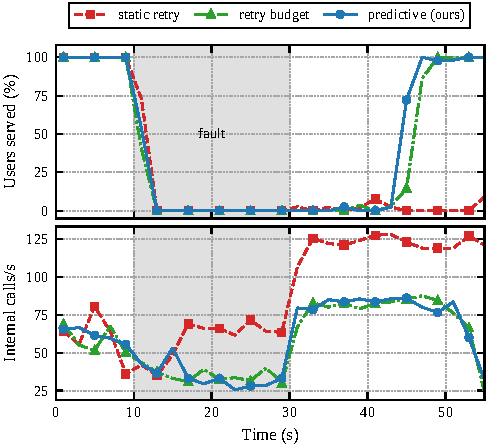
\includegraphics[width=\columnwidth]{plot_timeline.pdf}
\caption{Metastable experiment, run 1. Top: users served. Bottom: internal calls per second. Shaded: fault active. Static retries stay near 0\% after the fault while working harder than before it.}
\label{fig:meta}
\end{figure}

\begin{figure}[!t]
\centering
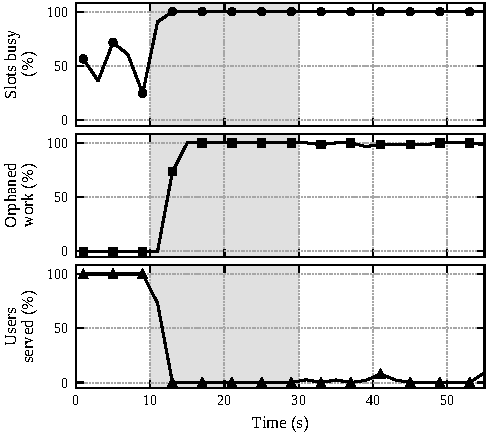
\includegraphics[width=\columnwidth]{plot_busy.pdf}
\caption{Static retries, metastable run 1 (shaded: fault active). Top to bottom: order's slots busy, share of order's finished work that was orphaned, users served. The slots are 100\% busy while almost no user is served: busy but no progress.}
\label{fig:busy}
\end{figure}

Against static retries the predictive controller's differences are clear ($p = 0.001$ for success after the fault, $p = 0.003$ for recovery time, $p < 0.001$ for calls). Against the budget the trend favours it but is not significant with five runs ($p = 0.059$, $0.091$ and $0.132$). Against the reactive controller success and recovery time are not significantly different ($p = 0.25$ and $0.31$), but the predictive controller made far fewer calls during the fault (661 against 974, $p < 0.001$) and the livelock did not form.

Fig.~\ref{fig:trace} shows the controller in one run. At 11.5\,s, 1.5\,s into the ramp, the risk on gateway$\to$order crossed 0.5 while congestion was starting below it, and the edge was cut from three attempts to two, while $\rho$ was still about 0, so no reactive rule could have fired. It was cut to one attempt at 13.5\,s. At 20.5\,s order$\to$payment developed its own storm and the reactive safety net cut it; it was restored at 33.5\,s. Gateway$\to$order was restored step by step at 50.5\,s and 53.5\,s. In all five runs the predictive controller made its first cut at 11.5\,s, while the reactive controller first cut at 17.5--19.5\,s, after the livelock had formed.

\begin{figure}[!t]
\centering
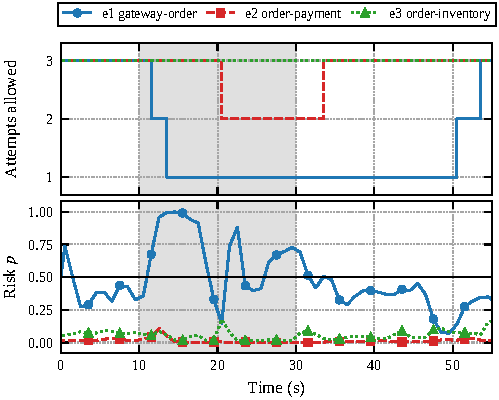
\includegraphics[width=\columnwidth]{plot_controller.pdf}
\caption{Predictive controller, metastable run 1 (shaded: fault active). Top: attempts allowed per edge. Bottom: predicted risk (line: threshold 0.5).}
\label{fig:trace}
\end{figure}

\subsection{Error Burst}
Table~\ref{tab:burst} shows the opposite situation. With fast failures and free slots each attempt is an independent chance: at the 70\% peak one attempt succeeds 30\% of the time, three attempts $1-0.7^3 \approx 66\%$. Static retry is therefore the best strategy (73.2\%) and no retry the worst (39.7\%). The fixed budget throws away useful retries (54.3\%, $p<0.001$ against predictive). The predictive controller kept 70.0\% (against 73.2\% for static, $p = 0.21$, not significant) with the fewest calls per successful user, because the congestion gate prevents cuts when there is no congestion. Every strategy recovered as soon as the fault ended, since a 1\,s queue leaves no orphans. Keeping retries has a cost: the 95th-percentile latency was about 3.2\,s against 0.7\,s for the budget.

\begin{table}[!t]
\caption{Error-Burst Experiment (5 Runs Each)}
\label{tab:burst}
\centering
\small
\setlength{\tabcolsep}{4pt}
\begin{tabular}{|L{1.55cm}|L{1.75cm}|L{0.95cm}|L{1.1cm}|L{1.15cm}|}
\hline
\textbf{Strategy} & \textbf{Success during fault} & \textbf{Calls} & \textbf{Calls per success} & \textbf{p95 latency} \\ \hline
No retry & 39.7 $\pm$ 1.5\% & 1,191 & 7.5 & 284 ms \\ \hline
Static retry & 73.2 $\pm$ 3.5\% & 1,699 & 5.7 & 4,031 ms \\ \hline
Budget 10\% & 54.3 $\pm$ 3.2\% & 1,363 & 6.4 & 663 ms \\ \hline
Reactive & 70.4 $\pm$ 1.0\% & 1,581 & 5.5 & 3,913 ms \\ \hline
Predictive & 70.0 $\pm$ 3.8\% & 1,493 & 5.3 & 3,156 ms \\ \hline
\end{tabular}
\end{table}

\subsection{Summary of Findings}
Fig.~\ref{fig:summary} and Table~\ref{tab:summary} put both experiments together. Every fixed policy is bad somewhere: no retry loses users when healthy, static retry never recovers from the metastable fault, and the budget discards useful retries in the error burst. The reactive controller fixes the storm only after it has formed. The predictive controller is the only strategy that is not bad in any column.

\begin{figure*}[!t]
\centering
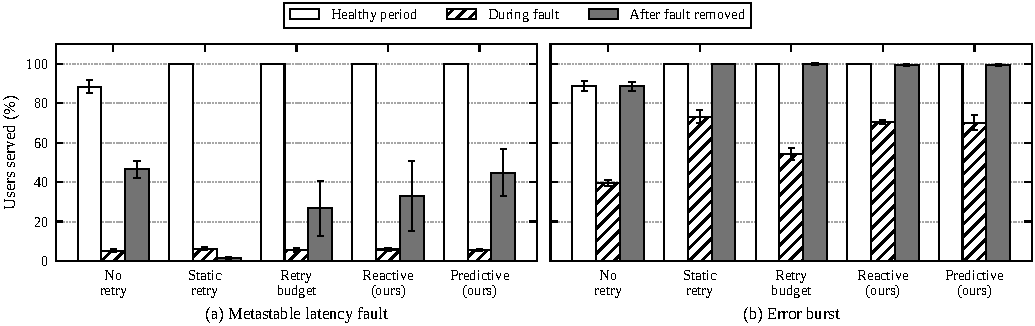
\includegraphics[width=\textwidth]{plot_summary.pdf}
\caption{Users served by the five strategies under both faults, in the healthy period, during the fault and after the fault is removed (bars: mean of 5 runs; whiskers: standard deviation).}
\label{fig:summary}
\end{figure*}

\begin{table}[!t]
\caption{No Fixed Policy Is Right for Both Faults}
\label{tab:summary}
\centering
\small
\begin{tabular}{|L{1.35cm}|L{1.2cm}|L{1.95cm}|L{1.35cm}|}
\hline
\textbf{Strategy} & \textbf{Healthy} & \textbf{Metastable fault} & \textbf{Error burst} \\ \hline
No retry & loses 11--12\% & recovers, 11.4 s & 39.7\% (worst) \\ \hline
Static retry & 100\% & never recovers & 73.2\% (best) \\ \hline
Budget 10\% & 100\% & 3 of 5, 20.0 s & 54.3\% \\ \hline
Reactive & 100\% & 4 of 5, livelock forms first & 70.4\% \\ \hline
Predictive & 100\% & 5 of 5, livelock never forms & 70.0\% \\ \hline
\end{tabular}
\end{table}

\subsection{Overall Results}
Table~\ref{tab:overall} collects the main result of every part of the project in one place.

\begin{table}[!t]
\caption{Overall Results}
\label{tab:overall}
\centering
\small
\setlength{\tabcolsep}{4pt}
\begin{tabular}{|L{1.45cm}|L{3.0cm}|L{2.85cm}|}
\hline
\textbf{Part} & \textbf{Measure} & \textbf{Result} \\ \hline
Dataset & runs, attempts, checks & 78 runs, 263,864 attempts, 6 of 6 checks pass \\ \hline
Detection & livelock windows; false alarms & 131 of 1,878; 0 of 636 healthy \\ \hline
Detection & user success, flagged vs other bad windows & 9.0\% vs 68.1\% \\ \hline
Prediction & accuracy; balanced accuracy & 91.8\%; 88.9\% \\ \hline
Prediction & F1; MCC; ROC-AUC & 0.75; 0.71; 0.95 \\ \hline
Prediction & early warning & 30 of 30 episodes, median 8\,s \\ \hline
Prediction & cost per prediction & 5.2\,$\mu$s \\ \hline
Control & metastable: recovered, static vs predictive & 0 of 5 vs 5 of 5 \\ \hline
Control & metastable: livelock formed & 5 of 5 vs 0 of 5 \\ \hline
Control & error burst: success, static / budget / predictive & 73.2\% / 54.3\% / 70.0\% \\ \hline
Live demo & last 5\,s served, run 1 vs run 2 & 0 of 80 vs 78 of 80 \\ \hline
\end{tabular}
\end{table}

%====================================================================
\section{Discussion}
\label{sec:disc}

\textbf{Retries are good or bad depending on capacity.} A retry against a service that fails fast and has spare slots is a free second chance; a retry against a saturated service adds to the queue that causes the failure. A fixed policy can only be tuned for one of these. The controller therefore needs a signal of \emph{congestion} (overload and rising latency below the edge), not just of failure, and our congestion-gate lesson confirms this.

\textbf{Acting early changes the outcome.} The reactive controller eventually fixes the storm, but by then a backlog of orphaned requests exists and has to drain. Cutting 1.5\,s into the ramp keeps that backlog small: the livelock never formed, and the controller made 32\% fewer calls during the fault than the reactive one.

\textbf{Per-edge analysis matters.} The storm forms where retries can pile up (gateway$\to$order), not where the fault is (payment). Graph features carry the first sign of trouble from the leaf edges upwards, which is why they matter most before onset.

\textbf{Operating-systems view.} The problem is the classical livelock and receive-livelock pattern moved from threads and interrupts to services: bounded worker pools (counting semaphores), bounded waiting, wasted work on abandoned requests, and feedback control in the style of TCP's AIMD. The Utilization Law and Little's Law both explain the storm and validate the data (for example, about 53 attempts/s each timing out at 2\,s gives about 107 calls in flight, close to the 100--105 measured in the storm windows).

%====================================================================
\section{Limitations and Future Work}
\label{sec:limits}

The testbed runs on one machine with Python threads and the Flask development server, so absolute capacities and latencies belong to this testbed; we report the mechanism (Eq.~\ref{eq:exit}) rather than only numbers. The call chain has two levels; amplification multiplies per level, so deeper chains would be worse and our numbers are a lower bound. The labels come from our own definition because no external ground truth for livelock exists; we validated them against user success, the fault timeline and a sensitivity sweep. The model is logistic regression rather than a temporal graph network~\cite{tgn2020}, and the random forest shows that a stronger model has headroom. The model was trained on data recorded under static retries while the controller changes the policy at run time, which shifts what the model sees; the reactive safety net and overload-based restoring limit the effect. Five runs per strategy is small, so we only claim clear differences. The gate's thresholds were chosen by replaying the first round of experiments, and all final numbers come from new runs. A fault inside order itself would only be caught by the reactive safety net. The risk values are not calibrated probabilities, and the order$\to$payment edge has too few positive windows to judge.

Future work includes a temporal graph model over longer histories, deeper call chains deployed across machines, dropping orphaned requests at the queue using the propagated deadline, learning the size of each cut, retraining on data recorded with the controller active, and validation on production traces if a dataset with per-attempt retry fields becomes available.

%====================================================================
\section{Conclusion}

We built a real four-service testbed in which retry storms form by themselves from an injected slowdown, and reproduced a self-sustaining livelock that a simple capacity inequality explains. We defined livelock formally per call edge, which found 131 livelock windows with no false alarms and matched what users experienced. We predicted livelock 2--12\,s ahead with 91.8\% accuracy, 88.9\% balanced accuracy and MCC 0.71 on runs the model never saw, warning before all 30 episodes with a median lead of 8\,s at about 5\,$\mu$s per prediction. Our predictive retry controller stopped the livelock from forming in all five runs and recovered in all five, while keeping close to static-retry success in an error burst. The main lesson is that retries help with short, fast failures and hurt during saturation, so the retry budget has to be controlled while the system runs, and preferably before the storm forms.

\appendices

\section{User Guide}
\textbf{Requirements.} Python 3.9 or newer on Windows, Linux or macOS. Install the libraries once with \texttt{python -m pip install -r requirements.txt} (Flask, requests, scikit-learn, scipy, networkx, matplotlib). On Linux or macOS use \texttt{python3}.

\textbf{Running the demonstration} (from the \texttt{code} folder, three terminals):\par\raggedright
\begin{enumerate}
\item \texttt{python -m unittest discover tests}: runs the 50 unit tests; the output ends with \texttt{OK}.
\item Terminal 1: \texttt{python run\_all.py} starts the four services and resets every configuration to healthy. It stops with Ctrl+C.
\item Terminal 2 (typed as one line):
\begin{footnotesize}
\begin{verbatim}
python scenario_runner.py --scenario_id live1
  --mode gradual --fault latency --queue_wait 10
  --normal_sec 10 --ramp_sec 10 --hold_sec 8
  --recovery_sec 25
\end{verbatim}
\end{footnotesize}
runs one fault scenario (53\,s). Then \texttt{python analyze\_run.py live1} prints the per-phase report (Fig.~\ref{fig:live}a).
\item \texttt{python labeling.py} applies the four conditions to the recorded dataset; \texttt{python prediction\_model.py} trains and tests the model; \texttt{python show\_metrics.py} prints the confusion matrix and metrics (Fig.~\ref{fig:metricsout}).
\item Terminal 3: \texttt{python controller.py --mode predictive --duration\_sec 90}, then immediately in Terminal 2 the same scenario command with \texttt{--scenario\_id live2}, and \texttt{python analyze\_run.py live2} (Fig.~\ref{fig:live}b). The controller prints one decision line per second and restores the original policy when it stops.
\item Optional: \texttt{python evaluate\_model.py} prints the full evaluation (intervals, calibration, cost) in about 45\,s; \texttt{python run\_pipeline.py} regenerates everything from scratch in about 1.5 hours (\texttt{--quick}: about 20 minutes).
\end{enumerate}

\textbf{Common problems.} ``Ports already in use'' means an old copy of the services is still running; close it. A scenario name can be used only once, so a repeated run needs a new name. ``Waiting for the previous run's leftover requests'' is normal after a long-queue run and clears within about 20\,s. Pressing Ctrl+C during a run removes the fault and marks the run as interrupted, and the analysis scripts ignore it.

\section{Project Structure}
\begin{itemize}
\item \texttt{code/services/}: the four services (gateway, order, payment, inventory).
\item \texttt{code/common/}: shared configuration, retry client, retry policy file, fault injection, telemetry, safe file writes.
\item \texttt{code/configs/}: the live fault settings each service reads on every request.
\item \texttt{code/*.py}: the scripts of Table~\ref{tab:modules}.
\item \texttt{code/tests/test\_core.py}: the 50 unit tests.
\item \texttt{code/data/}: the dataset: raw JSON-line logs of 78 runs, the scenario manifest, labelled windows and healthy baselines.
\item \texttt{code/results/}: every result file (detection, prediction, evaluation, experiments, validation, sensitivity), the trained \texttt{model.json} and all figures; \texttt{RESULTS.md} lists every number in one place.
\item \texttt{docs/}: question bank, code walkthrough and the public-dataset search.
\end{itemize}

%====================================================================
\begin{thebibliography}{99}

\bibitem{bronson2021} N. Bronson, A. Aghayev, A. Charapko, and T. Zhu, ``Metastable failures in distributed systems,'' in \emph{Proc. Workshop on Hot Topics in Operating Systems (HotOS)}, ACM, 2021, pp. 221--227.

\bibitem{huang2022} L. Huang, M. Magnusson, A. B. Muralikrishna, S. Estyak, R. Isaacs, A. Aghayev, T. Zhu, and A. Charapko, ``Metastable failures in the wild,'' in \emph{Proc. 16th USENIX Symp. on Operating Systems Design and Implementation (OSDI)}, 2022.

\bibitem{isaacs2025} R. Isaacs, P. Alvaro, R. Majumdar, K.-K. Muniswamy-Reddy, M. Salamati, and S. Soudjani, ``Analyzing metastable failures,'' in \emph{Proc. Workshop on Hot Topics in Operating Systems (HotOS)}, ACM, 2025.

\bibitem{haeberlen2025} A. Haeberlen, ``Modeling metastability,'' in \emph{Proc. Workshop on Hot Topics in Operating Systems (HotOS)}, ACM, 2025.

\bibitem{alvaro2025} P. Alvaro \emph{et al.}, ``Formal analysis of metastable failures in software systems,'' arXiv:2510.03551, 2025.

\bibitem{farahbakhsh2026} A. Farahbakhsh, Q. Lu, L. Alvisi, A. Haeberlen, and R. van Renesse, ``Characterizing metastable faults and failures,'' arXiv:2606.00942, 2026.

\bibitem{retryguard2025} J. Tavori, A. Bremler-Barr, H. Levy, and O. Lavi, ``RetryGuard: Preventing self-inflicted and attack-driven retry storms in cloud applications,'' arXiv:2511.23278, 2025.

\bibitem{brooker2019} M. Brooker, ``Timeouts, retries, and backoff with jitter,'' Amazon Builders' Library, 2019. [Online]. Available: aws.amazon.com/builders-library/timeouts-retries-and-backoff-with-jitter

\bibitem{breakwater2020} I. Cho, A. Saeed, J. Fried, S. J. Park, M. Alizadeh, and A. Belay, ``Overload control for $\mu$s-scale RPCs with Breakwater,'' in \emph{Proc. 14th USENIX OSDI}, 2020, pp. 299--314.

\bibitem{topfull2024} J. Park, J. Park, Y. Jung, H. Lim, H. Yeo, and D. Han, ``TopFull: An adaptive top-down overload control for SLO-oriented microservices,'' in \emph{Proc. ACM SIGCOMM}, 2024.

\bibitem{rajomon2025} J. Xing, A. Giannoukos, P. Loh, S. Wang, J. Qiu, H. M. Demoulin, K. Kallas, and B. C. Lee, ``Rajomon: Decentralized and coordinated overload control for latency-sensitive microservices,'' in \emph{Proc. 22nd USENIX NSDI}, 2025.

\bibitem{lee2024} I.-T. A. Lee, Z. Zhang, A. Parwal, and M. Chabbi, ``The tale of errors in microservices,'' \emph{Proc. ACM Meas. Anal. Comput. Syst. (SIGMETRICS 2025)}, vol. 8, no. 3, Art. 46, Dec. 2024.

\bibitem{seer2019} Y. Gan \emph{et al.}, ``Seer: Leveraging big data to navigate the complexity of performance debugging in cloud microservices,'' in \emph{Proc. ACM ASPLOS}, 2019, pp. 19--33.

\bibitem{firm2020} H. Qiu, S. S. Banerjee, S. Jha, Z. T. Kalbarczyk, and R. K. Iyer, ``FIRM: An intelligent fine-grained resource management framework for SLO-oriented microservices,'' in \emph{Proc. 14th USENIX OSDI}, 2020.

\bibitem{sage2021} Y. Gan, M. Liang, S. Dev, D. Lo, and C. Delimitrou, ``Sage: Practical and scalable ML-driven performance debugging in microservices,'' in \emph{Proc. ACM ASPLOS}, 2021.

\bibitem{ltfp2026} H. Zou, Y. Zhao, X. Chen, L. Wang, J. Yu, and L. Jiang, ``LTFP: Lead-time-aware failure prediction based on service GNNs for AIOps,'' \emph{Algorithms}, vol. 19, no. 9, Art. 720, 2026.

\bibitem{li2026} L. Li, ``Service dependency modeling and failure propagation prediction in distributed systems based on graph neural networks,'' \emph{Discover Artificial Intelligence}, vol. 6, Art. 512, 2026.

\bibitem{alibaba2021} S. Luo, H. Xu, C. Lu, K. Ye, G. Xu, L. Zhang, Y. Ding, J. He, and C. Xu, ``Characterizing microservice dependency and performance: Alibaba trace analysis,'' in \emph{Proc. ACM Symp. on Cloud Computing (SoCC)}, 2021.

\bibitem{meta2023} D. Huye, Y. Shkuro, and R. R. Sambasivan, ``Lifting the veil on Meta's microservice architecture: Analyses of topology and request workflows,'' in \emph{Proc. USENIX ATC}, 2023, pp. 419--432.

\bibitem{rcaeval2024} L. Pham, H. Zhang, H. Ha, F. Salim, and X. Zhang, ``RCAEval: A benchmark for root cause analysis of microservice systems with telemetry data,'' arXiv:2412.17015, 2024.

\bibitem{tgn2020} E. Rossi, B. Chamberlain, F. Frasca, D. Eynard, F. Monti, and M. Bronstein, ``Temporal graph networks for deep learning on dynamic graphs,'' arXiv:2006.10637, 2020.

\end{thebibliography}

\end{document}
